\documentclass[openany]{book}
\usepackage{amsmath,amssymb,amsthm}
\usepackage{graphicx,float} % Required for the inclusion of images
\usepackage{wrapfig}
\usepackage{caption}
\usepackage{subcaption}
\usepackage{cite}  			% BibTeX
\usepackage{makeidx} 		% For index
\usepackage[nottoc]{tocbibind}

\usepackage{hyperref}
\hypersetup{colorlinks,linkcolor=blue}

\usepackage[titletoc]{appendix}
\usepackage{bm}				% For bold greek letter
\usepackage{indentfirst}	% enable /indent
\usepackage{remreset}		% renumbering the sections

\usepackage{sectsty} 					% Allows your to change titles style
%    \chapterfont{\sffamily } 			% Delete the bold style and set the sans-serif font
    \allsectionsfont{\sffamily} 		% Delete the bold style and set the sans-serif font

\makeatletter
  \@removefromreset{section}{chapter}
\makeatother
\renewcommand{\thesection}{\arabic{section}}
%++++++++++++++++++++++++++++++++++++++++++

\interfootnotelinepenalty=10000 %enable longer length of footnote

\usepackage{titlesec} %Set the Section symbol
\titleformat{\section}{\normalfont\Large\bfseries}{\S\thesection}{1em}{}

%+++++++++++++++++++++++++++++++++++++++++++++++++++++
\title{AP Courses Review Notes\\AP3204\\Waves and Optics} % Title
\author{WU PEILIN \\ ~ \\
% 12-May-2017 14:00 to 16:00 \\
% AC2 1614 Lecture Theatre \\
% 0045
} % Author name
\makeindex
%+++++++++++++++++++++++++++++++++++++++++++++++++++++
\begin{document}
\frontmatter
\maketitle
\tableofcontents
\clearpage

\mainmatter
%\setcounter{page}{1}
\chapter{Vibration}
\section{Free Vibration}
\subsection{Simple Harmonic Motion}
A periodic motion is a motion which repeats itself after regular intervals of time, and the simplest kind of periodic motion is a \emph{simple harmonic motion}\index{simple harmonic motion} in which the displacement varies sinusoidally with time.

To understand simple harmonic motion, we consider a point $P$ rotating on the circumference of a circle of radius $a$ with an angular velocity $\omega $.
%\begin{figure}[h]
%\centering
%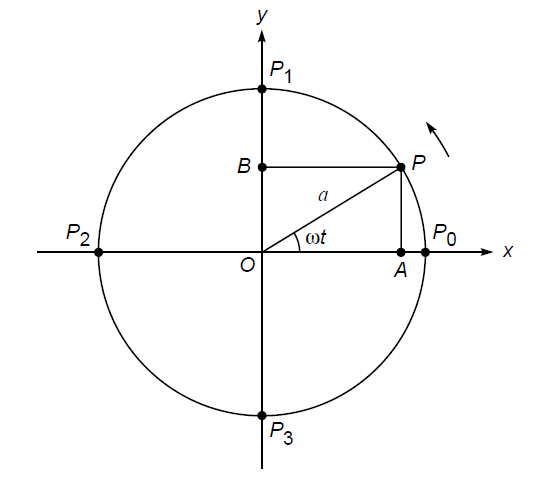
\includegraphics[width=0.3\textwidth]{Figure/1.PNG}
%\end{figure}
We can obtain the projection of Point $P$ on $x$ and $y$ axis and taking the initial phases into account:
\begin{align*}
x&=a\cos (\omega t+\theta)\\
y&=a\sin (\omega t+\theta),
\end{align*}
and the velocity:
\begin{align*}
v_x&=\dot{x}=-a\omega \sin (\omega t+\theta)=-\omega x\\
v_y&=\dot{y}=a\omega \cos (\omega t+\theta)=\omega y,
\end{align*}
and the acceleration:
\begin{align*}
a_x&=\ddot{x}=-a\omega ^2\cos (\omega t+\theta)=-\omega ^2x\\
a_y&=\ddot{y}=-a\omega ^2\sin (\omega t+\theta)=-\omega ^2y
\end{align*}

Here is a crucial observation about the acceleration, we have a second order differential equation:
\begin{equation}\label{eq:1}
\ddot{\mathbf{r}}=-\omega ^2\mathbf{r}
\end{equation}

Let's consider an alternative situation: A mass $m$ attached to a spring with stiffness $k$. With initial position deviate from the equilibrium position, mass $m$ will exhibits periodic motion with the net exerted by spring as a \emph{linear restoring force}\index{Linear restoring force}
\[\mathbf{F}=-k\mathbf{x},\]
and with the \emph{Newton's second law}\index{Newton's second law} of motion
\[\mathbf{F}=m\mathbf{a}.\]
Therefore,
\[m\mathbf{a}=\mathbf{F}=-k\mathbf{x}.\]
Thus we have the following equation similar to the equation \eqref{eq:1}
\begin{equation}\label{eq:2}
\ddot{\mathbf{x}}+\left(\sqrt{\frac{k}{m}}\right)^2\mathbf{x}=0
\end{equation}
We can see that $\omega = \sqrt{\frac{k}{m}}$. Actually, the original circle is the phase diagram of simple harmonic motion. Moreover, it is important to state that: An object exhibits simple harmonic motion if the net external force acting on it is a linear restoring force.

Following the deduction, we obtain the general solution to simple harmonic motion:
\[x=A\sin \left(\sqrt{\frac{k}{m}}t+\phi \right),\]
where $A$ is the maximum amplitude, $k$ is the stiffness of spring, $m$ is the mass and $\phi $

Let's consider the energy of this simple mechanics system. 
\[
E_{total}=\underbrace{E_0\sin ^2\omega t}_\text{Potential Energy}+\underbrace{E_0\cos ^2\omega t}_\text{Kinetic Energy}
\]

According to the \emph{principle of superposition}\index{Principle of superposition}, any oscillation can be modelled as a composition of multiple or infinite simple harmonic motion components.
\subsection{Fourier Theorem}
\emph{Fourier Theorem}\index{Fourier Theorem}\footnote{You can think of that what Fourier Theorem actually states is to decompose original infinite vector space into the linear combination of two sets of orthogonal infinite vector space thus correspondingly, the element naturally following the decomposition. And those two orthogonal vector spaces rely on the orthogonality of triangular functions $f=C\sin (nx)$ and $g=C'\cos (mx)$.} states that any periodic function can be expressed as a sum of the sine and cosine functions whose frequencies increase in the ratio of natural numbers.

Any periodic function $f(t)$ with period $T$ ($f(t+nT)=f(t)$ with $n\in \mathbb{N}$) can be expanded in the form wit1h $\omega =\frac{2\pi}{T}$:
\begin{equation}\label{eq:3}
f(t)=\frac{1}{2}a_0+\sum _{n=1}^{\infty}a_n \cos (n\omega t)+\sum _{n=1}^{\infty}b_n \sin (n\omega t),
\end{equation}
with coefficient series determined by \footnote{The coefficients $a_n$ and $b_n$ can be easily determined by
using the following properties of the trigonometric functions:
\begin{align*}
\int _{t_0}^{t_0+T}\cos n\omega t\cos \omega m\omega t&=\begin{cases}
0&\text{if } m\neq n\\
\frac{T}{2}&\text{if }m=n\neq 0\\
T&\text{if }m=n=0
\end{cases}\\
\int _{t_0}^{t_0+T}\sin n\omega t\sin \omega m\omega t&=\begin{cases}
0&\text{if } m\neq n\\
\frac{T}{2}&\text{if }m=n\neq 0\\
T&\text{if }m=n=0
\end{cases}\\
\int _{t_0}^{t_0+T}\sin n\omega t\cos \omega m\omega t&=0
\end{align*}
}

\begin{align*}
a_n&=\frac{2}{T}\int _{t_0}^{t_0+T}f(t)\cos n\omega t\,dt\\
b_n&=\frac{2}{T}\int _{t_0}^{t_0+T}f(t)\sin n\omega t\,dt
\end{align*}
%Therefore, the full expansion of a periodic function with Fourier series is
%\begin{align*}
%f(t)&=\frac{1}{2}a_0\\
%&+\sum _{n=1}^{\infty}\left(\frac{2}{T}\int _{t_0}^{t_0+T}f(t)\cos n\omega tdt\right) \cos (n\omega t)\\
%&+\sum _{n=1}^{\infty}\left(\frac{2}{T}\int _{t_0}^{t_0+T}f(t)\sin n\omega tdt\right)\sin (n\omega t).
%\end{align*}
\subsection{Other Cases of Simple Harmonic Motion}
\subsubsection{Simple Pendulum}
For simple pendulum, the linear restoring force $\mathbf{F}= - mg \bm \theta $, and the acceleration $\mathbf{a}=L \ddot{\bm\theta}$, thus:
\[\mathbf{F}=-mg \bm{\theta }=mL \ddot{\bm\theta}\quad \Rightarrow \quad\ddot{\bm{\theta}}+\left(\sqrt{\frac{g}{L}}\right)^2\bm{\theta}=0,\]
which gives:
\[\ddot{\theta }+\left(\sqrt{\frac{g\sin \theta }{L}}\right)^2\theta =0.\]

However, this is not simple harmonic motion unless we make approximation that within small range that $\sin \theta =\theta $,
\[\ddot{\theta }+\left(\sqrt{\frac{g}{L}}\right)^2\theta =0\]
\[\theta =\Theta \sin (\sqrt{\frac{g}{L}} t+\phi ).\]

\subsubsection{Compound Pendulum}
Quite similar to simple pendulum,
\[\ddot{\theta}+\frac{mg}{J}\frac{L}{2} \sin \theta=0\]
% another error

with same approximation $\sin \theta =\theta $, we have $\omega =\sqrt{\frac{mgL}{2J}}$
\subsubsection{Torsional Pendulum}
The linear restoring force $\mathbf{F}=-c\bm{\theta}$, followed by $-c\theta =J\ddot{\theta}$,
\[\ddot{\theta}+\frac{c}{J}\theta=0\]

therefore, $\omega =\sqrt{\frac{c}{J}}$, $\theta =\Theta \sin \left(\sqrt{\frac{c}{J}} t+\phi \right)$
\section{Damped Vibration}
For damped vibration, one big difference is that there is an additional first order force $\mathbf{F}_r$, $\mathbf{F}=\mathbf{F}_0+\mathbf{F}_r=-kx-r\dot{\mathbf{x}}$. Its physical interpretation gives the first order resistance or friction contributing to the continuous energy dissipation and decay of amplitude. Again by Newton's second law, $\mathbf{F}=m\ddot{\mathbf{x}}$,

\begin{equation}\label{eq:4}
\ddot{\mathbf{x}}+\underbrace{\frac{r}{m}}_{\gamma }\dot{\mathbf{x}}+\underbrace{\frac{k}{m}}_{\omega _0}\mathbf{x}=0
\end{equation}

Denote $\beta =\frac{\gamma}{2}$, $\alpha _{1,2}=-\beta \pm \sqrt{\beta ^2-\omega _0^2}$, we have the general solution: $x=Ce^{\alpha _1t}+C'e^{\alpha _2t}$.
\subsection{Light Damping}
If $\beta <\omega _0$ ($\alpha _{1,2}\in \mathbb{C}$), which means that the retarding force is small compared with the restoring force, we called it \emph{light damping}\index{Light damping}, thus gives an exponential decaying sinusoidal wave $\sin (\omega _ft+\phi )$ enveloped by decaying amplitude $A_0e^{-\beta t}$.
\[x=\underbrace{A_0e^{-\beta t}}_\text{Amplitude}\sin (\underbrace{\sqrt{\omega _0^2-\beta ^2}}_{\omega _f} t+\phi )\]
\subsection{Critical Damping}
If $\beta =\omega _0$ ($\alpha _{1,2}=-\beta $) meaning the retarding force reaches the restoring force in the spring, we called it \emph{critical damping}\index{Critical damping}. 
\[x=A_0e^{-\beta t}\]

Noted: Critical damping has the quickest return to equilibrium.
\subsection{Heavy Damping}
If $\beta >\omega _0$ ($\alpha _{1,2}\in \mathbb{R}$), in this case, the medium is so viscous that the retarding force is greater then the restoring force.
\[x=Ce^{\alpha _{1,2}t}\]

Noted: There is no oscillation but only overdamped curve. And surely it is the most boring one among those three, it just simply return to its original position.
\subsection{Quantify Damping}
Since three cases have differently behaviours, we want to quantify the quality of damping, etc. Here is some factors to describe decays due to damping
\begin{enumerate}
\item Width: $\gamma =\frac{r}{m}$
\item Logarithmic decrement: $\delta =\ln \frac{A_1}{A_2}$
\item Quality factor: $Q=\frac{\omega _0}{\gamma}$ (For a lightly damping system, $Q<0.5$)
\end{enumerate}

\section{Forced Vibration}
Despite the linear restoring force and retarding force, there is also a periodic force angular frequency $\omega $ $\mathbf{F}_p=\mathbf{F}_0\sin \omega t$, following the same deduction,

\begin{equation}\label{eq:5}
\ddot{\mathbf{x}}+\underbrace{\frac{r}{m}}_{\gamma =2\beta}\dot{\mathbf{x}}+\underbrace{\frac{k}{m}}_{\omega _0}\mathbf{x}=\underbrace{\frac{\mathbf{F}_0}{m}}_{P}\sin \omega t
\end{equation}

We immediately notice that equation \eqref{eq:4} is the homogeneous equation for equation \eqref{eq:5}, therefore, general solution of equation \eqref{eq:4} is the contemporary solution of equation \eqref{eq:5}. Here we want to find the particular solution to equation \eqref{eq:5}, $x_p=B\sin (\omega t-\delta )$, where 

\begin{align*}
\delta &=\arctan \left(\frac{2\beta \omega }{\omega _0^2-\omega ^2}\right)\\
B &=\frac{P}{\sqrt{\left(\omega _0^2-\omega ^2\right)^2+4\beta ^2\omega ^2}}\\
P &={F_0}/{m}
\end{align*}

Therefore, the general solution for force damping system:
\[x=\overbrace{\underbrace{A_0e^{-\beta t}}_\text{Amplitude}\sin (\underbrace{\sqrt{\omega _0^2-\beta ^2}}_{\omega _f} t+\phi )}^\text{Damping term}+\overbrace{\underbrace{\frac{{F_0}/{m}}{\sqrt{\left(\omega _0^2-\omega ^2\right)^2+4\beta ^2\omega ^2}}}_{B}\sin (\omega t-\underbrace{\arctan \left(\frac{2\beta \omega }{\omega _0^2-\omega ^2}\right)}_{\delta })}^\text{Particular Solution}\]

\subsection{Steady State}
After damping term goes to zero, we have steady state solution, or physically interpreted as the response to the periodic force.

\[F=F_0\sin \omega t \quad \to \quad x=B\sin (\omega t-\delta )\]

\subsection{Resonance and Q factor}
For lightly damped motion, amplitude $B$ reaches its maximum at resonance. Therefore, we obtain $\omega _r=\sqrt{\omega _0^2-2\beta ^2}$ is the resonance frequency\footnote{For comparison: $\omega _r<\omega _f<\omega _0$} ($\omega _f=\sqrt{\omega _0^2-\beta ^2}$), and the amplitude for resonance is
\[B_r=\frac{F/m}{2\beta \sqrt{\omega _0^2-\beta ^2}}\]

Furthermore, we can define another evaluation factor $Q=\frac{\omega _0}{\gamma }=\frac{\omega _0}{2\beta }$. The larger the value of $Q$, the less the dissipative effect and the greater the number of free oscillation for given decrease of amplitude. And the amplitude for resonance with $B_0=\frac{F_0}{m\omega _0^2}=\frac{F_0}{k}$ is

\[B_r=\frac{F/m}{2\beta \sqrt{\omega _0^2-\beta ^2}}=\frac{\frac{F_0}{m\omega _0^2}}{\frac{2\beta }{\omega _0}\beta \sqrt{1-\frac{\beta ^2}{\omega _0^2}}}=\frac{B_0Q}{\sqrt{1-\frac{1}{4Q^2}}}\]

\subsection{Power Consumption}
Power is given by 
\[P=\mathbf{F}\cdot \mathbf{v}=\mathbf{F}\cdot \dot{\mathbf{x}}=F_0\sin \omega t \frac{d}{dt}\left(B\sin (\omega t-\delta )\right)=F_0B\omega \sin \omega t\cos (\omega t-\delta )=P(\omega )\]

The mean power within period is given by\footnote{The derivation following some crucial integral and $\delta $:
\[\int _{0}^{T}\sin \omega t\cos \omega tdt=0,\qquad \int _{0}^{T}\sin ^2\omega tdt=\frac{T}{2},\qquad \tan \delta =\frac{2\beta \omega }{\omega _0^2-\omega ^2}\]}
\[\bar{P}=\frac{F_0B\omega }{T}\int _{0}^{T}\sin \omega t\cos (\omega t-\delta )dt=\frac{F_0^2\omega ^2B}{m\left((\omega _0^2-\omega ^2)^2+4\omega ^2\beta ^2\right)}=\bar{P}(\omega )\]

We continue to make observation, 
\[\bar{P}(\omega )=\frac{F_0^2B}{m\left(\frac{(\omega _0^2-\omega ^2)^2}{\omega ^2}+4\beta ^2\right)}\]

We get maximun mean power $\bar{P}_{max}=\frac{F_0^2}{4m\beta }$ when $\omega =\omega _0$

In terms of quality factor, we can re-express the mean power as\footnote{Refer to the previous definition: $k=m\omega _0^2$}
\[\bar{P}=\frac{F_0^2\omega ^2B}{m\left((\omega _0^2-\omega ^2)^2+4\omega ^2\beta ^2\right)}=\frac{{F_0^2\omega ^2}/{2kQ}}{\left(\frac{\omega _0}{\omega }-\frac{\omega }{\omega _0}\right)^2+4\beta ^2}\]

\subsection{Bandwidth}
Since the mean power is the a function respect to $\omega $, we can draw $P-\omega $ graph. Within that graph, we further define that the width of the line segment at $\frac{1}{2}\bar{P}_{max}$ is bandwidth $\gamma $.\footnote{This result rises from non-trivial derivation:

\[\bar{P}=\frac{1}{2}\bar{P}_{max} \Rightarrow \left(\frac{\omega _0}{\omega }-\frac{\omega }{\omega _0}\right)^2+\frac{1}{Q^2}=\frac{2}{Q^2}\]

Making the approximation that $\frac{\omega _0}{\omega }-\frac{\omega }{\omega _0}\approx 2\frac{\omega _0-\omega}{\omega _0}$, we obtain that $\omega =\omega _0\pm \frac{\omega _0}{2Q}=\omega _0\pm \beta$, therefore gives that $\Delta \omega =\gamma$. Moreover, even if you did not make the approximation, the result is the same, because the second term in roots will cancel each out in the last subtraction. }

\subsection{Principle of Superposition}
Principle of superposition\footnote{Actually, principle of superposition for multiple periodic force naturally rises from the linear combination of the particular solutions corresponding to different source terms.} states that if two or more driving forces act on a system the response will equal the vector sum of the responses for each force acting alone.

\chapter{Wave Models}
\section{Wave Equation}
A wave is a disturbance of a continuous medium that propagates with fixed shape at constant velocity. How would you represent such an object mathematically? In a simple scenario, a wave is generated by shaking one end of a taut
string. Let's consider a simple property that the possible mathematical expression of wave should apply. Denote $f(z,t)$ as the displacement of the string at point $z$ at time $t$ and the initial position $g(z)=f(z,0)$
\[f(z,t)=f(z-vt,0)=g(z-vt)\]

That statement captures (mathematically) the essence of wave motion. It tells us that the function $f(z, t)$, which might have depended on $z$ and $t$ in the very special combination $z-vt$.

Based on that, wave equation gives mathematical description for waves and automatically admits as solution as all function of the form $f(z,t)=g(z-vt)$\footnote{The most general solution to wave equation is of the form
\[\Psi (z,t)=f(z-vt)+g(z+vt)\]},
\begin{equation}\label{eq:6}
\underbrace{\nabla ^2\Psi }_\text{Force}=\underbrace{\frac{1}{v^2}\frac{\partial ^2}{\partial t^2}\Psi}_\text{Inertia}
\end{equation}

\subsection{Derivation of Wave Function}
\subsubsection{Transverse Waves}
Let's derive wave equation for one-dimensional case. For wave on a string (transverse waves) with linear density $\rho $ and the string tension $T$ (for a small angle $\theta $) as figure \ref{fig2} shows
\begin{figure}[H]
\centering
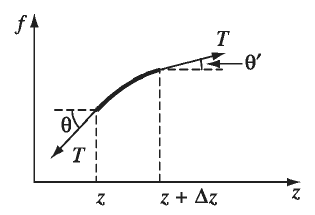
\includegraphics[width=0.45\textwidth]{Figure/2.PNG}
\caption{String segment}
\label{fig2}
\end{figure}
\[\Delta F=T(\sin \theta '-\sin \theta )\sim T(\tan \theta '-\tan \theta )\sim T\left(\left.\frac{\partial f}{\partial z}\right|_{z+\Delta z}-\left.\frac{\partial f}{\partial z}\right|_{z}\right)\sim T\frac{\partial ^2f}{\partial z^2}\Delta z\]

Newton's second law says: $\Delta F=\rho \Delta z\frac{\partial ^2f}{\partial t^2}$, therefore gives the wave equation: 
\begin{equation}
\frac{\partial ^2f}{\partial z^2}=\frac{\rho }{T}\frac{\partial ^2f}{\partial t^2}
\end{equation}

and high dimension follow the same derivation. 

Notice, in this case, the propagating speed $v=\sqrt{\frac{T}{\rho }}$

For simplicity, we usually consider sinusoidal wave of the form $z=A\sin (kx-\omega t+\phi )$\footnote{By convention, we denote $k=\frac{2\pi }{\lambda }$ and called it \emph{angular wave number}\index{Angular wave number}, $\omega =\frac{2\pi }{T}$ and called it \emph{angular frequency}\index{Angular frequency}, and $\nu =\frac{1}{T}$ as \emph{harmonic frequency}\index{Harmonic frequency}, by this
\[v=\lambda \nu=\frac{\lambda }{T}=\frac{\omega }{k}\]}
\subsubsection{Longitudinal Waves}
First consider the following spring model as shown by figure \ref{fig:3}, an array of little weights of mass m interconnected with massless springs of length $h$. The springs have a spring constant of $k$:
\begin{figure}[H]
\centering
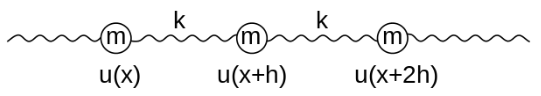
\includegraphics[scale=1]{Figure/3.PNG}
\caption{Springs system}
\label{fig:3}
\end{figure}
Here the dependent variable $u(x)$ measures the distance from the equilibrium of the mass situated at $x$, so that $u(x)$ essentially measures the magnitude of a disturbance (i.e. strain) that is travelling in an elastic material. The forces exerted on the mass $m$ at the location $x+h$ are:
\[F_{\mathit{Newton}}=m \cdot a(t)=m \cdot {{\partial^2 \over \partial t^2}u(x+h,t)}\]
\[F_\mathit{Hooke} = F_{x+2h} - F_x = k \left [ {u(x+2h,t) - u(x+h,t)} \right ] - k[u(x+h,t) - u(x,t)]\]

The equation of motion for the weight at the location $x+h$ is given by equating these two forces:
\[{\partial^2\over \partial t^2} u(x+h,t) = {k\over m}[u(x+2h,t)-u(x+h,t)-u(x+h,t)+u(x,t)]\]
where the time-dependence of $u(x)$ has been made explicit.

If the array of weights consists of $N$ weights spaced evenly over the length $L = Nh$ of total mass $M = Nm$, and the total spring constant of the array $K = k/N$ we can write the above equation as:
\[{\partial^2 \over \partial t^2} u(x+h,t)={KL^2 \over M}{u(x+2h,t)-2u(x+h,t)+u(x,t) \over h^2}\]

Taking the limit $N \to \infty$, $h \to \infty$ and assuming smoothness one gets:
\begin{equation}\label{eq:7}
{\partial^2 u(x,t) \over \partial t^2}={KL^2 \over M}{ \partial^2 u(x,t) \over \partial x^2 }
\end{equation}

Then, we can continue to apply it on continuous medium, for instance stress pulse in a bar. In the case of a stress pulse propagating through a beam the beam acts much like an infinite number of springs in series and can be taken as an extension of the equation derived for Hooke's law.

A beam of constant cross section made from a linear elastic material has a stiffness $K$ given by $K= {EA \over L}$, where $A$ is the cross sectional area and $E$ is the Young's modulus of the material. The wave equation becomes
\[{\partial^2 u(x,t) \over \partial t^2}={EAL \over M}{ \partial^2 u(x,t) \over \partial x^2 }\]

$AL$ is equal to the volume of the beam and therefore ${AL \over M}= {1 \over \rho}$ where $\rho$is the density of the material. The wave equation reduces to
\begin{equation}\label{eq:w2}
{ \partial^2 u(x,t) \over \partial x^2 }={ \rho\over E}{\partial^2 u(x,t) \over \partial t^2}
\end{equation}

The speed of a stress wave in a beam is therefore $v=\sqrt{E \over \rho}$.\footnote{From this, it is clear that wave speed is fixed by material properties}

%Quick summary:
%\begin{itemize}
%\item Transverse Waves: $\frac{\partial ^2f}{\partial z^2}=\frac{\rho }{T}\frac{\partial ^2f}{\partial t^2},\quad v=\sqrt{\frac{T}{\rho }}$
%\item Longitudinal Waves: ${ \partial^2 u \over \partial x^2 }={ \rho\over E}{\partial^2 u \over \partial t^2},\quad v=\sqrt{E \over \rho}$
%\end{itemize}
\subsection{Impedance of Stretched String}
When a transverse wave propagates in a string, the string offers certain opposition to the propagation of wave. This opposition is known as \emph{impedance}\index{Impedance}\footnote{$T=\rho v^2$} \footnote{Make it clear that the maximum transverse force is not $T$, but proportional to $T$} \footnote{From this you can see that impedance is only depend on the material properties} \footnote{Mechanics Impedance: \[F(\omega )=Z(\omega )v(\omega )\]}. 
\[Z=\frac{\text{maximum transverse force}}{\text{maximum transverse velocity}}=\frac{T}{v}=\rho v=\sqrt{T\rho }\]
\subsubsection{Derivation of Impedance}
\begin{wrapfigure}{L}{0.45\textwidth}
  \vspace{-20pt}  
  \begin{center}
    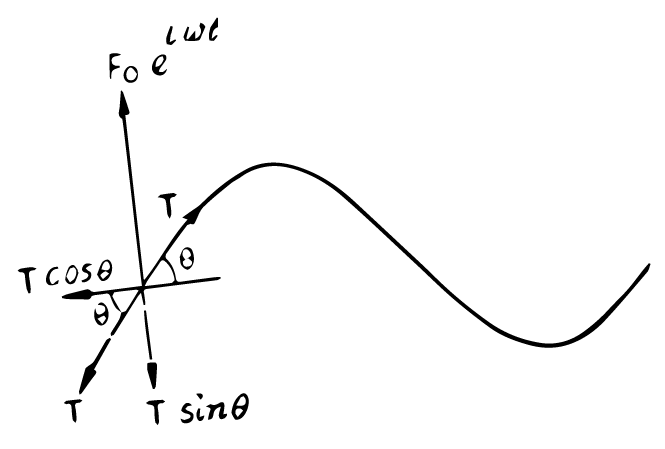
\includegraphics[width=0.4\textwidth]{Figure/5.PNG}
  \end{center}
  \vspace{-20pt}    
  \caption{Impedance}
\end{wrapfigure}
Here is the derivation of impedance:
\[Z=\frac{\text{maximum transverse force}}{\text{maximum transverse velocity}}=\frac{T}{v}\]

Consider applying an alternating force $F=F_0e^{i\omega t}$ to a string where $F_0$ is amplitude of $F$ and $\omega $ is the angular frequency of this alternating force. $T$ is he constant force acting throughout the length of string. 

As shown left, making approximaion, for a small enough angle $\theta $
\[F_0e^{i\omega t}=-T\sin \theta \to -T\tan \theta =-T\frac{\partial \psi (z,t)}{\partial z}\]
Since our wave function is $\psi (z,t)=Ae^{i(\omega t-kz)}$, therefore, $\frac{\partial \psi (z,t)}{\partial z}=-ikAe^{i(\omega t-kz)}$. At the end $z=0$
\[F_0e^{i\omega t}=-T\left(-ikAe^{i\omega t}\right)\Rightarrow F_0=ikTA\]

But $k={\omega \over v}$, therefore, $A=\frac{F_0v}{iT\omega }$, thus $\psi (z,t)=\frac{F_0v}{iT\omega }e^{i(\omega t-kz )}$. The transverse velocity is given by
\[V=\dot{\psi }=\frac{F_0v}{T}e^{i(\omega t-kz )}\Rightarrow V_{max}=\frac{F_0v}{T}\]

and for the maximum transverse force $F_{max}=F_0$, therefore, 
\[Z=\frac{\text{maximum transverse force}}{\text{maximum transverse velocity}}=\frac{F_0T}{F_0v}=\frac{T}{v}=\rho v=\sqrt{T\rho }\] 
\subsection{Transport of Power}
Wave in a stretched string carries energy. And the \emph{transport energy}\index{Transport energy} of a string is given by the \emph{kinetic energy}\index{Kinetic energy} of string segment of length $\Delta z$:
\[\Delta E=\frac{1}{2}\Delta mV_{max}^2=\frac{1}{2}\rho \omega ^2A^2\Delta z\quad (V_{max}=A\omega )\]

Since the rate of transfer of energy is given by the product of energy of unit length and velocity of propagation of wave, therefore rate of transfer of energy, or \emph{power}\index{Power}, will be
\[P=\frac{1}{2}\rho \omega ^2A^2v=\frac{1}{2}Z\omega ^2A^2\]
\section{Wave at Boundary}
\subsection{Reflection and Transmission}
A boundary divides regions of different impedance, an incident wave propagates at boundary will be both reflected and transmitted forming \emph{reflective wave}\index{Reflective wave} and \emph{transmitted wave}\index{Transmitted wave}.

Denote that the incident wave function is $\psi _i=A_ie^{i(\omega t-k_1z)}$, reflective wave as $\psi =B_re^{i(\omega t+k_1z)}$, and transmitted wave as$\psi =A_te^{i(\omega t-k_2z)}$ and then $f_i(t-\frac{x}{v_1})=\psi _i$, $f_r(t+\frac{x}{v_1})=\psi _r$, and $f_t(t-\frac{x}{v_1})=\psi _t$.
\subsubsection{Derivation of Reflective and Transmission Coefficients}
\begin{wrapfigure}{L}{0.3\textwidth}
  \vspace{-20pt}  
  \begin{center}
    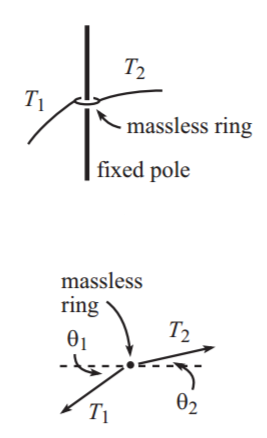
\includegraphics[width=0.25\textwidth]{Figure/4.PNG}
  \end{center}
  \vspace{-20pt}    
  \caption{Boundary}
  \vspace{-0pt} 
\end{wrapfigure}
First, let's consider the boundary condition at $x=0$ between two different densities. The string is continuous, thus for all $t$,\footnote{Denote $\frac{\partial f}{\partial z}=f'$ and $\frac{\partial f}{\partial t}=\dot{f}$} 
\begin{equation}\label{eq:8}
\psi _L(0,t)=\psi _R(0,t)\Rightarrow f_{i}(t)+f_{r}(t)=f_{t}(t)
\end{equation}
this condition gives that
\begin{equation}\label{eq:10}
A_i+B_r=A_t
\end{equation}
and the slope is continuous, thus:
\begin{equation}\label{eq:9}
{\partial \psi _L(z,t)\over \partial z|_{z=0}}={\partial \psi _R(z,t)\over \partial z|_{z=0} }\Rightarrow -\frac{f_i'(t)}{v_1}+\frac{f_r'(t)}{v_1}=-\frac{f_t'(t)}{v_2}
\end{equation}
or $v_2f_i(t)-v_2f_r(t)=v_1f_t(t)$.

Then, consider the scenario as shown in the left, the net transverse force on the massless ring must also be zero to avoid infinite acceleration, This condition gives $T_1\sin \theta_1=T_2\sin \theta_2$, by approximation $\sin \theta \to \tan \theta$ when $\theta$ is small enough,
\[T_1\left.\frac{\partial \psi _L(z,t)}{\partial z}\right|_{z=0}=T_2\left.\frac{\partial \psi _R(z,t)}{\partial z}\right|_{z=0}\]
Noted, the tension within string is equal $T_1=T_2$, then it reduces to the \emph{first boundary condition}\index{First boundary condition} \eqref{eq:8}. Then with tension now distinct, consider the \emph{second boundary condition}\index{Second boundary condition} \eqref{eq:9}, the equation convert into
\[-\frac{f_i'(t)}{v_1}T_1+\frac{f_r'(t)}{v_1}T_1=-\frac{f_t'(t)}{v_2}T_2\Rightarrow -f_i'(t)Z_1+f_r'(t)Z_1=-f_t'(t)Z_2\]

therefore,
\begin{align*}
-ik_1A_ie^{i(\omega t-k_1z)}Z_1+ik_1B_re^{i(\omega t+k_1z)}Z_1&=-ik_2A_te^{i(\omega t-k_2z)}Z_2\\
-k_1A_ie^{i\omega t}Z_1+k_1B_re^{i\omega t}Z_1&=-k_2A_te^{i\omega t}Z_2\quad (z=0)
\end{align*}
\begin{equation}\label{eq:11}
-k_1A_iZ_1+k_1B_rZ_1=-k_2A_tZ_2
\end{equation}

combining \eqref{eq:10} and \eqref{eq:11}, we can determine the \emph{reflection coefficient}\index{Reflection coefficient} and \emph{transmission coefficient}\index{Transmission coefficient}
\begin{align*}
R&\equiv \frac{B_r}{A_i}=\frac{v_2-v_1}{v_2+v_1}=\frac{Z_1-Z_2}{Z_1+Z_2}=\frac{\sqrt{\rho _1}-\sqrt{\rho _2}}{\sqrt{\rho _1}+\sqrt{\rho _2}}\\
T&\equiv \frac{A_t}{A_i}=\frac{2v_2}{v_2+v_1}=\frac{2Z_1}{Z_1+Z_2}=\frac{2\sqrt{\rho _1}}{\sqrt{\rho _1}+\sqrt{\rho _2}}
\end{align*}
\subsubsection{Reflection and Transmission of Power}
\begin{enumerate}
\item \emph{Reflection coefficient of power}\index{Reflection coefficient of power}
\[\frac{\text{Reflected power}}{\text{Incident power}}=\frac{\frac{1}{2}Z_1\omega ^2B_r^2}{\frac{1}{2}Z_1\omega ^2A_i^2}=R^2=\left(\frac{Z_1-Z_2}{Z_1+Z_2}\right)^2\]
\item \emph{Transmission coefficient of power}\index{Transmission coefficient of power}
\[\frac{\text{Transmitted power}}{\text{Incident power}}=\frac{\frac{1}{2}Z_2\omega ^2A_t^2}{\frac{1}{2}Z_1\omega ^2A_i^2}=T^2=\left(\frac{2Z_1}{Z_1+Z_2}\right)^2\]
\end{enumerate}
\subsection{Image Waves}
The most general solution to wave equation  \eqref{eq:6} is of the form
\[\Psi (z,t)=f(z-vt)+g(z+vt)\]

its physical interpretation is clear that every solution satisfies wave equation can be decomposed into a wave moving to right $f(z-vt)$ and a wave moving to left $g(z+vt)$.

Applying this idea, we can explain wave reflection at a fixed end quite clearly, please refer to figure \ref{fig:6}
\begin{figure}[H]
\centering
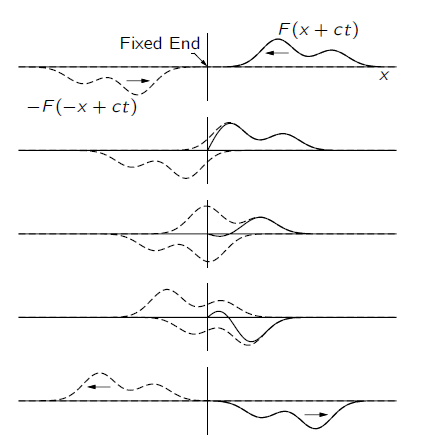
\includegraphics[scale=1]{Figure/6.PNG}
\caption{Reflection of a wave as a superposition of two travelling waves.}
\label{fig:6}
\end{figure}
\section{Hygens' Principle}
Like all waves, light can be viewed as a series of crests and trough moving away from a source.

A \emph{ray}\index{Ray} is an arrow drawn perpendicular to a wave front that points in the direction of the wave’s motion.
\subsection{Huygens' Principle}
Huygens' theory is essentially based on a geometrical construction which allows us to determine the shape of the wave front at any time, if the shape of the wave front at an earlier time is known. A \emph{wave front}\index{Wave front} is the locus of the points which are in the same phase.

Now, according to \emph{Huygens' principle}\index{Huygens' principle}\footnote{Huygens' principle can be seen as a consequence of the homogeneity of space — the space is uniform in all locations. Any disturbance created in a sufficiently small region of homogeneous space (or in a homogeneous medium) propagates from that region in all geodesic directions. The waves created by this disturbance, in turn, create disturbances in other regions, and so on. The superposition of all the waves results in the observed pattern of wave propagation.}, each point of a wave front is a source of secondary disturbance, and the wavelets emanating from these points spread out in all directions with the speed of the wave. The envelope of these wavelets gives the shape of the new wave front.

\subsection{Principle of Reversibility}
The path of a ray of light through any
system is completely reversible.

\section{Wave Behaviours}
\subsection{Reflection and Transmission}
\subsection{Refraction}
\subsection{Interference}
Superposition principle states that when two or more waves move in the same linear medium, the net displacement of the medium at any point equals the algebraic sum of the wave functions of the individual waves.
\subsubsection{Harmonic Waves}
Consider two waves, denoted as $\psi _1(z,t)=A_0\sin (kz-\omega t)$ and $\psi _2(z,t)=A_0\sin (kz-\omega t -\phi)$, have same travelling direction with same amplitude and frequency only having phase difference $\phi $ are called \emph{harmonic waves}\index{Harmonic waves}. The interference between two harmonic waves
\[\psi (z,t)=\psi _1(z,t)+\psi _2(z,t)=A_0\sin (kz-\omega t)+A_0\sin (kz-\omega t -\phi)=2A_0\cos \frac{\phi }{2}\sin (kz-\omega t-\frac{\phi }{2})\]

Therefore, we can see that after the interference, the amplitude becomes $A=2A_0\cos \frac{\phi }{2}$, and the path difference between the two waves can be determined by $\Delta z=\frac{\phi}{2\pi}\lambda $
\subsubsection{Standing Waves}
A \emph{standing wave}\index{Standing wave}\footnote{Strictly speaking, standing wave is not a wave because it doesn't satisfy wave equation \eqref{eq:6}.} can be produced in a string due to the interference of two sinusoidal waves with equal amplitude and frequency traveling in opposite directions, denoted as $\psi _i(z,t)=A_0\sin (kz-\omega t)$ and $\psi _r(z,t)=A_0\sin (kz+\omega t)$. The interference between these two sinusoidal waves gives the standing waves
\[\psi (z,t)=\psi _i(z,t)+\psi _r(z,t)=A_0\sin (kz-\omega t)+A_0\sin (kz+\omega t)=2A_0\sin kz\cos \omega t \]

For standing wave, there are two situation that is worthy to consider:

\paragraph{Standing wave in a string fixed as both end }

First, let's make some definitions. The string has a number of natural patterns of vibration, called \emph{normal modes}\index{Normal modes}. Each normal mode has a \emph{characteristic frequency}\index{Characteristic frequency}. The lowest of these frequencies is called the \emph{fundamental frequency}\index{Fundamental frequency}, which together with the higher frequencies form a \emph{harmonic series}\index{harmonic series}. \emph{Antinodes}\index{Antinodes} are points of maximum displacement, while
\emph{nodes}\index{Nodes} are points of zero displacement.

Since both end are fixed, therefore, the total string length must be the multiple of half of the wavelength $L=n\frac{\lambda _n}{2},\ (n\in \mathbb{N})$, and for the frequency, we have the relation\footnote{Since $v=\frac{\omega _n}{k_n}=\lambda _n\nu _n=\sqrt{T\rho }$} that $\nu _n=\frac{nv}{2L}=\frac{n}{2L}\sqrt{T\rho }$.

\paragraph{Standing waves in air columns (fixed end or open end)} 
Sound sources can be used to produce longitudinal standing waves in air columns.The phase relationship between incident and reflected waves depends on whether or not the reflecting end of the air column is open or closed.
\begin{enumerate}
\item an open pipe

For the wave length, since one end is open, therefore, at both end\footnote{If you want to generate sound wave, the start node is also an open end thus force to be an antinode.}, it has to be an antinode meaning the total pipe length is multiple of the half of the wavelength, $L=n\frac{\lambda _n}{2},\ (n\in \mathbb{N})$, thus referring to the longitudinal wave equation \eqref{eq:w2}, we can derive the frequency $\nu _n=\frac{nv}{2L}=\frac{n}{2L}\sqrt{E/\rho }$
\item a closed pipe

For the wave length, since one end is closed, therefore, at the end\footnote{If you want to generate sound wave, the start node is also an open end thus force to be an antinode.}, it has to be a node meaning the total pipe length is multiple of the quarter of the wavelength, $L=n\frac{\lambda _n}{4},\ (n=2k+1, \text{where }k\in \mathbb{N})$, thus referring to the longitudinal wave equation \eqref{eq:w2}, we can derive the frequency $\nu _n=\frac{nv}{4L}=\frac{n}{4L}\sqrt{E/\rho }$
\end{enumerate}


\subsection{Beats}
\emph{Beats}\index{Beats} are formed by the combination of two waves of equal amplitude but slightly different frequencies travelling in the same direction. Denote the two waves as $\psi _1(z,t)=A_0\cos (\omega _1t-k_1z)$ and $\psi _2(z,t)=A_0\cos (\omega _2t-k_2z)$. By the superposition principle, we have the interference as shown by \ref{fig:7},
\begin{align*}
\psi &=\psi_1+\psi _2=A_0\cos (\omega _1t-k_1z)+A_0\cos (\omega _2t-k_2z)\\
&=\underbrace{2A_0\cos \left(\frac{\omega _1-\omega _2}{2}t-\frac{k_1-k_2}{2}z\right)}_\text{Amplitude modulation}\underbrace{\cos \left(\frac{\omega _1+\omega _2}{2}t-\frac{k_1+k_2}{2}z\right)}_\text{Travelling wave part}
\end{align*}

\begin{figure}[H]
\centering
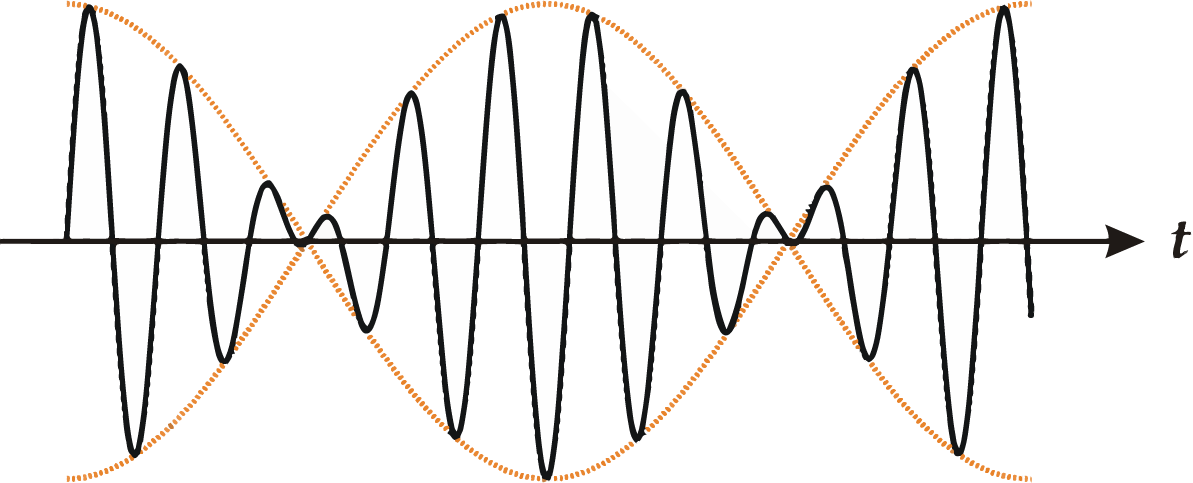
\includegraphics[width=0.45\textwidth]{Figure/7.PNG}
\caption{Beats}
\label{fig:7}
\end{figure}

\subsection{Wave Packet}
\subsubsection{Group Velocity and Phase Velocity}
Continue with the beats, let's redenote the wave equation that $\psi _1=A_0\sin (kz-\omega t)$ and $\psi _2=A_0\sin \left((k+\Delta k)z-(\omega +\Delta \omega)t\right)$. Their superposition gives the waveform as shown by \ref{fig:7},
\[\psi =\psi_1+\psi_2=\underbrace{2A_0\cos \left(\frac{\Delta \omega }{2}t-\frac{\Delta k}{2}z\right)}_\text{Modulated
amplitude}\underbrace{\sin \left((k+\frac{\Delta k}{2})z-(\omega +\frac{\Delta \omega }{2})t\right)}_\text{sine wave}\]

Notice right now, we have two different wave velocity, one is the \emph{phase velocity}\index{Phase velocity} $v_p$ defined as  the rate at which the phase of the wave propagates in space, and the other is \emph{group velocity}\index{Group velocity} $v_g$ defined as the velocity with which the overall shape of the waves' amplitudes — known as the modulation or \emph{envelope}\index{Envelope} of the wave — propagates through space.

\begin{equation}\label{eq:12}
v_p=\frac{\lambda }{T}=\frac{\omega }{k}
\end{equation}
\begin{equation}\label{eq:13}
v_g=\frac{\Delta \omega }{\Delta k}=\frac{d\omega (k)}{dk}
\end{equation}

\paragraph{An alternative approach}
A wave package is the superposition of a bunch of harmonic
waves, which can be written as $f(x,t)\sum_\nu a_\nu 
\cos(2\pi\nu)\left(t-\frac{x}{v(\nu)}\right)$, where 
$\nu$ is the frequency. The position of the center of the
package is the coordinate where the amplitude is the maximal,
so we can differentiate with $\nu$\footnote{The next maximal is
the same as $(x,t)=(0,0)$, as time passing, at that position,
all the phase angles of all the components should be the same,
just like the scene of $(x,t)=(0,0)$.}:
\[\frac{d}{d\nu}[\nu(t-\frac{x}{v(\nu)})]=0.\]
Simplify, we have $t=x\frac{d}{d\nu}(\frac{\nu}{v})$, thus 
$V_g=\frac{x}{t}=\frac{d\nu}{d(\frac{1}{\lambda})}=\frac{d\omega}{dk}$\footnote{This approach is said to be used by Fermi. From: 
\url{https://www.zhihu.com/question/56142122}.}.

\subsubsection{Non-dispersive and Dispersive Waves}
If a travelling wave is losing energy, then it called \emph{dispersive waves}\index{Dispersive waves} and those does not are called \emph{non-dispersive waves}\index{Non-dispersive waves}.

In non-dispersive waves\footnote{This is for the wave travelling in vacuum only.}, all components travel at the same speed: $v_p=\frac{\omega }{k}=\text{constant}$.

In dispersive waves\footnote{This is true for waves travelling in a medium other than vacuum.}, components travel at different speeds: $v_p=\frac{\omega (k)}{k}$, thus we use group velocity $v_g=\frac{d\omega (k)}{dk}$

\chapter{Sound Waves - Longitudinal Waves}
\section{Longitudinal Waves}
Please refers to the derivation of longitudinal wave equation \eqref{eq:w2} in \S 4.1.
\begin{equation}
{\partial^2 u(x,t) \over \partial x^2 }={ \rho\over E}{\partial^2 u(x,t) \over \partial t^2}
\end{equation}

where $u(x,t)$ is the particle displacement\footnote{Noted that: by generalization, if we denote that the \emph{particle displacement}\index{Particle displacement} as \[\delta (\mathbf{r},t)=\delta \cos \left(\mathbf{k}\cdot \mathbf{r}-\omega t+\psi _{\delta ,0}\right)\]
the \emph{particle velocity}\index{Particle velocity} is determined by
\[v(\mathbf{r},t)=\frac{\partial \delta (\mathbf{r},t)}{\partial t}=\omega \delta \cos \left(\mathbf{k}\cdot \mathbf{r}-\omega t+\psi _{\delta ,0}+\frac{\pi }{2}\right)=v_0\cos \left(\mathbf{k}\cdot \mathbf{r}-\omega t+\psi _{v,0}\right)\] 

and the amplitude of the \emph{acoustic pressure}\index{Acoustic pressure}
\[p(\mathbf{r},t)=-B\frac{\delta (\mathbf{r},t)}{\partial x}=-\rho v^2\frac{\delta (\mathbf{r},t)}{\partial x}=\rho c^2\mathbf{k}_x\delta \cos \left(\mathbf{k}\cdot \mathbf{r}-\omega t+\psi _{\delta ,0}+\frac{\pi }{2}\right)=p_0\cos \left(\mathbf{k}\cdot \mathbf{r}-\omega t+\psi _{p,0}\right)\]

and the amplitude of the specific \emph{acoustic impedance}\index{Acoustic impedance} is given by (using Laplace transform)
\[z(\mathbf{r},s)=\left|\hat{z}(\mathbf{r},s)\right|=\left|\frac{\hat{p}(\mathbf{r},s)}{\hat{v}(\mathbf{r},s)}\right|=\left|\frac{p_0}{v_0}\frac{\frac{s\cos \psi _{v,0}-\omega \sin \psi _{v,0}}{s^2+\omega ^2}}{\frac{s\cos \psi _{p,0}-\omega \sin \psi _{p,0}}{s^2+\omega ^2}}\right|=\frac{p_0}{v_0}=\frac{\rho v^2k_x}{\omega }=\rho v\]}.

Here gives another more directly derivation:

By hooks' law $\text{Applying stress}= \text{Elastic modulus} \times \text{Strain to the segment}$ or $\frac{F}{A}=E\frac{\partial u(x,t)}{\partial x}$, thus:
\[\frac{\partial F}{\partial x}=EA\frac{\partial ^2u(x,t)}{\partial x^2}\]

by Newton's second law: 
\[F(x+\Delta x)-F(x)=\frac{\partial F}{\partial x}\Delta x=EA\Delta x\frac{\partial ^2u(x,t)}{\partial x^2}=m\ddot{x}=\rho A\Delta x\frac{\partial ^2u(x,t)}{\partial t^2}\]

thus, we obtain ${\partial^2 u(x,t) \over \partial x^2 }={ \rho\over E}{\partial^2 u(x,t) \over \partial t^2}$, with wave speed $v=\sqrt{\frac{E}{\rho}}$
\section{Sound Speed}
\subsection{Sound Speed in Liquid and Gas Media}
Sound wave speed $v$ depends on the bulk modulus $B$ and equilibrium density $\rho $ of the medium.

Therefore, in the liquid, the sound wave speed is determined by
\[v=\sqrt{\frac{B}{\rho }}\quad \text{where }B=-\frac{\Delta P}{\Delta V/V}\]

In the gas, the sound wave speed is determined by
\[v=\sqrt{\frac{\gamma P}{\rho}}\]

where $\gamma =\frac{c_p}{c_v}$ is \emph{characteristic parameter}\index{Characteristic parameter} - the ratio of the specific heat at constant pressure to the specific heat at constant volume. 

If it is an ideal gas, by applying ideal gas law's corollary $PM=\rho RT$, we can re-express the equation in terms of the absolute temperature $T$ and molar mass $M$.
\[v=\sqrt{\frac{\gamma RT}{M}}\]
\section{Harmonic Sound Waves}
For displacement wave function $u(x,t)=u_0\cos (kx-\omega t)$, its corresponding pressure can be determined by $\Delta P=\Delta P_{max}\sin (kx-\omega t)=-B\frac{\partial u(x,t)}{\partial x}=-Bku_0\sin (kx-\omega t)$, therefore, we have that The displacement and the pressure variation are out of phase by $\frac{\pi }{2}$.

The pressure amplitude is proportional to the displacement amplitude.
\[\Delta P_{max}=Bku_0=\rho v\omega u_0\]
\section{Sound Wave Intensity and Intensity Level}
\subsection{Intensity}
Sound wave intensity\footnote{Both $\mathbf{I}$ and $\mathbf{v}$ are vectors, which means that both have a direction as well as a magnitude. The direction of sound intensity is the average direction in which energy is flowing.} is defined as $\mathbf{I}=p\mathbf{v}=\rho v(\omega A_0)^2$, the multiple of sound pressure and particle velocity. 

The average sound intensity during time $T$ is given by $<\mathbf{I}>=\frac{1}{T}\int _{0}^{T}p(t)\mathbf{v}(t)dt$, thus for wave as $u(x,t)=u_0\cos (kx-\omega t)$
\begin{align*}
<I>&=\frac{1}{T}\int _{0}^{T}p(t)v(t)dt\\
&=\frac{1}{T}\int _{0}^{T}\rho v\omega ^2u_0^2\sin ^2(kx-\omega t)dt\\
&=\frac{1}{2}\rho v(\omega u_0)^2=\frac{p_0^2}{2\rho v}=\frac{p_0^2}{2Z}
\end{align*}
\subsection{Sound Intensity Level (SIL)}
A logarithmic intensity level scale is defined using a \emph{reference intensity}\index{Reference intensity} $I_0$\footnote{Threshold of hearing $I_0=10^{-12}W/M^2$.}
\begin{equation}
\beta =10\log \frac{I}{I_0}\ (dB)
\end{equation}

\section{Doppler Effect}
The change in frequency heard by an observer whenever there is relative motion between the source and the observer is called \emph{Doppler effect}\index{Doppler effect}.

By conventional assumptions, the observer is in the left hand side the source is in the right hand side. And sign conventional denote right as $+$ and left as $-$ for both observer and source speed.
\begin{equation}\label{eq:doppler effect}
f'_o=f_s\left(\frac{v_{\text{wave speed}}\pm v_{\text{observer speed}}}{v_{\text{wave speed}}\pm v_{\text{source speed}}}\right)
\end{equation}
\subsection{Shock Waves}
\emph{Shock waves}\index{Shock waves} are produced when a sound source moves through a medium with a speed $v_s$ which is greater than the wave speed.
\[\sin \theta =\frac{v}{v_s}\]

The shock wave front has a conical shape with a half angle which depends on the Mach number of the source, defined as the ratio $\frac{v_s}{v}$.

\chapter{Light Waves - Electromagnetic Waves}
\section{Maxwell's Equations}
\begin{subequations}
Maxwell's equations (In general):
\begin{align}
	&\nabla \cdot \mathbf{E}=\frac{\rho}{\varepsilon_0}\quad &\textrm{Gauss' Law} \\
            &\nabla \cdot \mathbf{B}= 0\quad &\textrm{Gauss' Law ($\mathbf{B}$ Fields)}\\
          &\nabla \times \mathbf{E}=-\frac{\partial \mathbf{B}}{\partial t}\quad &\textrm{Faraday's Law}\\
          &\nabla \times \mathbf{B}=\mu_0 \mathbf{J} + \mu_0\varepsilon_0\frac{\partial \mathbf{E}}{\partial t}\quad &\textrm{Ampere's Law} 
\end{align}

\indent Maxwell's equations (In matter):
\begin{align}
	&\nabla \cdot \mathbf{D}=\rho _f\quad &\textrm{Gauss' Law} \\
            &\nabla \cdot \mathbf{B}= 0\quad &\textrm{Gauss' Law ($\mathbf{B}$ Fields)}\\
          &\nabla \times \mathbf{E}=-\frac{\partial \mathbf{B}}{\partial t}\quad &\textrm{Faraday's Law}\\
          &\nabla \times \mathbf{H}=\mathbf{J}_f+\frac{\partial \mathbf{D}}{\partial t}\quad &\textrm{Ampere's Law} 
\end{align}
\end{subequations}
\subsection{Derivation of Speed of Light}
\subsubsection{Electric Field Equation}
\begin{align*}
\nabla \times \nabla \times \mathbf{E}&=\nabla \times \left(-\frac{\partial \mathbf{B}}{\partial t}\right)=\frac{\partial }{\partial t}\left(\nabla \times \mathbf{B}\right)\\
&=\frac{\partial \mu_0 \mathbf{J}}{\partial t}+\mu_0 \varepsilon_0\frac{\partial }{\partial t}\frac{\partial \mathbf{E}}{\partial t}\\
\nabla ^2\mathbf{E}&=\mu_0 \varepsilon_0\frac{\partial ^2 \mathbf{E}}{\partial t^2}
\end{align*}

This is a wave equation, have the electric wave travels at the speed of $c=\sqrt{\mu_0\varepsilon_0}$
\subsubsection{Magnetic Field Equation}
\begin{align*}
\nabla \times \nabla \times \mathbf{B}&=\nabla \times \left(\mu_0 \mathbf{J} + \mu_0\varepsilon_0\frac{\partial \mathbf{E}}{\partial t}\right)\\
&=\mu_0 \nabla \times \mathbf{J}+\mu_0\varepsilon_0 \nabla \times \frac{\partial \mathbf{E}}{\partial t}=-\mu_0\varepsilon_0 \frac{\partial }{\partial t}\left(\nabla \times \mathbf{E}\right)\\
\nabla ^2\mathbf{B}&=-\mu_0\varepsilon_0 \frac{\partial }{\partial t}\left(-\frac{\partial \mathbf{B}}{\partial t}\right)=\mu_0\varepsilon_0 \frac{\partial ^2\mathbf{B}}{\partial t^2}
\end{align*}

This is, again, a wave equation, have the magnetic wave travels at the speed of $c=\frac{1}{\sqrt{\mu_0\varepsilon_0 }}$
\subsection{Light as Electromagnetic Waves}
For speed of light equals to the phase speed of electric wave as well as magnetic waves suggests a profound nature that light is an electromagnetic waves. 
\[\begin{cases}
\nabla ^2\mathbf{E}=\mu_0 \varepsilon_0\frac{\partial ^2 \mathbf{E}}{\partial t^2}\\
\nabla ^2\mathbf{B}=\mu_0\varepsilon_0 \frac{\partial ^2\mathbf{B}}{\partial t^2}
\end{cases}\]
\subsection{Conservation Laws}
\subsubsection{Continuity Equation}
Consider the conservation law of charge, formally the charge in a volume $\Omega $ is 
\[Q(t)=\int _{\Omega }\rho (\mathbf{r},t)d\tau\]

by the local conservation law,
\[\frac{dQ}{dt}=-\oint _{\S}\mathbf{J}\cdot d\mathbf{a}\]

invoking divergence theorem and $Q(t)$,
\[\int _{\Omega }\frac{\partial \rho (\mathbf{r},t)}{\partial t}=-\int _{\Omega }\nabla \cdot \mathbf{J}\Rightarrow \frac{\partial }{\partial t}\rho (\mathbf{r},t)=-\nabla \cdot \mathbf{J}\]

This is the \emph{continuity equation}\index{Continuity equation} - the precise mathematical statement of local conservation of charge. The purpose of this chapter is to develop the corresponding equations for local conservation of energy and momentum.
\subsubsection{Energy and Energy Density (Poynting's Theorem)}
From the electrostatics and magnetostatics, we have that
\[\begin{cases}
W_e=\frac{\varepsilon _0}{2}\displaystyle\int E^2d\tau\\
W_m=\frac{1}{2\mu _0}\displaystyle\int B^2d\tau
\end{cases}\]

Suggesting that $W_{em}=W_e+W_m$, and the total energy in electromagnetic fields, per unit volume, or should called it as \emph{energy density}\index{Energy density},is,
\[u=\frac{1}{2}\left(\varepsilon _0E^2+\frac{1}{\mu_0}B^2\right)\]

Suppose we have some charge and current configuration which, at time t, produces fields $\mathbf{E}$ and $\mathbf{B}$. In the next instant, $dt$, the charges move around a bit.
\[\mathbf{F}\cdot d\mathbf{l}=q(\mathbf{E}+\mathbf{v}\cdot \mathbf{B})\cdot \mathbf{v}dt=q\mathbf{E}\cdot \mathbf{v}dt\]

so the rate at which work is done on all the charges in a volume $\Omega $ is
\[\frac{dW}{dt}=\int _{\Omega }\mathbf{E}\cdot \mathbf{J}\ d\tau \]

Thus we can see that $\mathbf{E}\cdot \mathbf{J}$ is the work done per unit time, per unit volume, which is to say, the power delivered per unit volume or \emph{energy flux}\index{Energy flux}. 

Then, by using Ampere-Maxwell law, we can eliminate $\mathbf{J}$
\[\mathbf{E}\cdot \mathbf{J}=\frac{1}{\mu_0}\mathbf{E}\cdot (\nabla \times \mathbf{B})-\varepsilon_0\mathbf{E}\cdot \frac{\partial \mathbf{E}}{\partial t}\]

and by invoking Faraday's law ($\nabla \times \mathbf{E}=-\frac{\partial \mathbf{B}}{\partial t}$) and product rule $\nabla \cdot \left(\mathbf{E}\times \mathbf{B}\right)=\mathbf{B}\cdot \left(\nabla \times \mathbf{E}\right)-\mathbf{E}\cdot \left(\nabla \times \mathbf{B}\right)$,
\[\mathbf{E}\cdot (\nabla \times \mathbf{B})=-\mathbf{B}\cdot \frac{\partial \mathbf{B}}{\partial t}-\nabla \cdot (\mathbf{E}\times \mathbf{E})\]

as $\mathbf{B}\cdot \frac{\partial \mathbf{B}}{\partial t}=\frac{1}{2}\frac{\partial }{\partial t}(B^2)$ and $\mathbf{E}\cdot \frac{\partial \mathbf{E}}{\partial t}=\frac{1}{2}\frac{\partial }{\partial t}(E^2)$, so
\[\mathbf{E}\cdot \mathbf{J}=-\frac{1}{2}\frac{\partial }{\partial t}\left(\varepsilon _0E^2+\frac{1}{\mu_0}B^2\right)-\nabla \cdot (\frac{1}{\mu _0}\mathbf{E}\times \mathbf{B})\]

applying the divergence theorem to the second term again, we obtain that:
\[\frac{dW}{dt}=-\frac{d}{dt}\int _{\Omega }\underbrace{\frac{1}{2}\left(\varepsilon _0E^2+\frac{1}{\mu_0}B^2\right)}_{u\text{ energy density}}d\tau - \oint _{S}\underbrace{\left(\frac{1}{\mu _0}\mathbf{E}\times \mathbf{B}\right)}_{\mathbf{S}\text{ flux density}}\cdot d\mathbf{a}\]

where $S$ is the surface bounding $\Omega $, this is \emph{Poynting's theorem}\index{Poynting's theorem}, it is the "work - energy theorem" of electrodynamics. 

Poynting's theorem says, then, that the work done on the charges by the electromagnetic force is equal to the decrease in energy remaining in the fields, less the energy that flowed out through the surface.

The energy per unit time, per unit area, transported by the fields is called the \emph{Poynting vector}\index{Poynting vector}:
\[\mathbf{S}\equiv \frac{1}{\mu _0}\mathbf{E}\times \mathbf{B}\]

Therefore, making these definitions, we can simplify Poynting's theorem:
\[\frac{dW}{dt}=-\frac{d}{dt}\int _{\Omega }ud\tau - \oint _{S}\mathbf{S}\cdot d\mathbf{a}\]

consider no work is done on the charges in $\Omega $ which $dW/dt=0$, thus
\[\int \frac{\partial u}{\partial t}d\tau =-\oint \mathbf{S}\cdot d\mathbf{a}=-\int (\nabla \cdot \mathbf{S}d\tau )\]

and hence
\[\frac{\partial u}{\partial t}=-\nabla \cdot \mathbf{S}\]

This is the "continuity equation" for energy - $u$ (energy density) plays the role of $\rho $ (charge density), and $\mathbf{S}$ takes the part of $\mathbf{J}$ (current density). It expresses local conservation of electromagnetic energy. 

\subsubsection{Momentum}
Let us consider a linearly polarized electromagnetic wave propagating in the $+z$ direction; we assume the electric field to be along the $x$ direction and the magnetic field along the $y$ direction. The electromagnetic wave is assumed to interact with a charge $q$; the electric field makes the charge move up and down along the $x$ axis.

Thus the charge acquires a certain velocity in the $x$ direction, and since the magnetic field is along the $y$ axis, a force $\mathbf{F}=q\mathbf{v}\times \mathbf{B}$ acts on the charge $q$. This force acts along the z axis (along the direction of propagation of the wave) and constitutes what is known as \emph{radiation pressure}\index{Radiation pressure}. Thus, $\mathbf{F}=qvB\hat{\mathbf{z}}$, since $B=\mu _0H=\frac{E}{c}$, we obtain $\mathbf{F}=\frac{qEv}{c}\hat{\mathbf{z}}$. Now $qEv$ represents the work done by the field on the charge per unit time; thus, then $\mathbf{F}=\frac{1}{c}\frac{dU}{dt}\hat{\mathbf{z}}$, where $U$ is total work done by the field.

But the force is equal to the change in momentum per unit time; consequently, the momentum per unit volume associated with the plane wave is given by
\[\mathbf{p}=\frac{U}{c}\hat{\mathbf{z}}\]

and by the Newton's law, the pressure $P$, applying the divergence theorem:
\[P=\frac{F}{A}=\frac{1}{cA}\frac{\partial U}{\partial t}=\frac{S}{c}\]
\subsection{Plane Electromagnetic Wave}
\subsubsection{Wave Function}
The simplest solution is given by plane electromagnetic wave:
\[ \begin{cases}
\mathbf{E}&=E_{max}\cos (kx-\omega t+\phi)\\
\mathbf{B}&=B_{max}\cos (kx-\omega t+\phi)
\end{cases} \]

where $c=\frac{\omega }{k}=\lambda f$. 
\begin{figure}[H]
\centering
\label{fig:8}
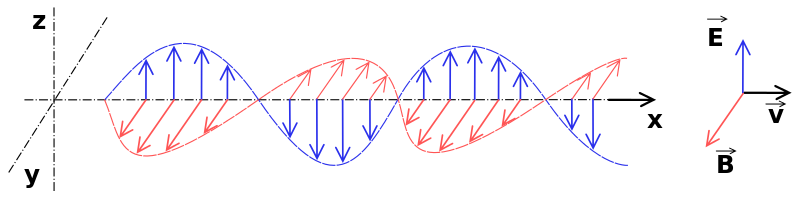
\includegraphics[scale=0.4]{Figure/8.PNG}
\caption{Plane electromagnetic wave}
\end{figure}
For plane electromagnetic wave, there are some basic properties:
\begin{itemize}
\item Electromagnetic waves obey the principle of superposition
\item $\mathbf{E}$ and $\mathbf{B}$ in the empty space is related by the following equation: $\frac{E}{B}=c$\footnote{Refer to the Poynting vector}

\begin{proof}
First, we can express the electromagnetic wave as the following form:
\begin{align*}
\mathbf{E}(\mathbf{r},t) &= \mathbf{E}_0 ~ e^{i(\mathbf{k}\cdot  \mathbf{r} - \omega t)}\\
\mathbf{B}(\mathbf{r},t) &= \mathbf{E}_0 ~ e^{i(\mathbf{k}\cdot  \mathbf{r} - \omega t)}
\end{align*}

then we consider the Faraday's law:
\[\nabla \times \mathbf{E}=-\frac{\partial \mathbf{B}}{\partial t}\]
\begin{align*}
\nabla \times \mathbf{E}&=\nabla \times \Bigl( \mathbf{E}_0 ~ e^{i(\mathbf{k}\cdot  \mathbf{r} - \omega t)} \Bigl)\\
&= i \mathbf{k}\times \mathbf{E}_0 ~ e^{i(\mathbf{k}\cdot  \mathbf{r} - \omega t)}\\
\partial \mathbf{B}(\mathbf{r},t) / \partial t&=- i \omega \mathbf{B}_0 ~ e^{i(\mathbf{k}\cdot  \mathbf{r} - \omega t)}
\end{align*}

Thus we can see that:
\[\mathbf{k} \times \mathbf{E}_0 = \omega ~ \mathbf{B}_0\]

For uniform plane electromagnetic wave, the relation simplifies itself into the following:
\[E_0=\frac{\omega }{k}B_0=cB_0\]
\end{proof}
\end{itemize}

Therefore, for the simplest case, the energy per unit volume associated with a plane wave is given by:
\[u=\frac{1}{2}\varepsilon _0E^2+\frac{1}{2}\frac{B^2}{\mu _0}\]

Furthermore, for linearly polarized plan wave,
\[u=\frac{1}{2}\varepsilon _0E^2\cos ^2(kx-\omega t)+\frac{1}{2}\frac{B^2}{\mu _0}\cos ^2(kx-\omega t)\] 

since $E_0=\frac{\omega }{k}B_0=cB_0$, we have that $\frac{1}{2}\varepsilon _0E^2=\frac{1}{2}\frac{B^2}{\mu _0}$, meaning the energy associated with the electric field is equal to the energy associated with the magnetic field. If we take the time average of the $\cos ^2$ terms, we get $u=\varepsilon _0E^2\cos ^2(kx-\omega t)=\frac{B^2}{\mu _0}\cos ^2(kx-\omega t)$,
\[<u>=\frac{1}{2}\varepsilon _0E^2=\frac{1}{2}\frac{B^2}{\mu _0}\]

Further, to obtain the intensity of the beam, we must multiply $<u>$ by the speed of propagation, which will give us the energy crossing a unit area in unit time. Thus, the intensity is given by
\begin{align*}
I&=\frac{1}{2}\varepsilon _0cE_0^2=\frac{1}{2}\sqrt{\frac{\varepsilon _0}{\mu _0}}E_0^2
\end{align*}

\subsection{Spherical Electromagnetic Waves}
\subsubsection{Wave Function}
For the spherical waves, the wave equation can be rewritten as
\[\frac{\partial ^2(ru)}{\partial t^2}=v^2\frac{\partial ^2(ru)}{\partial \mathbf{r}^2}\]
therefore, $u(\mathbf{r},t)=Ae^{i(\omega t\pm \mathbf{k}\cdot \mathbf{r})}$, thus it follows the inverse square law:
\[I=|u(\mathbf{r},t)|^2=\frac{|A|^2}{r^2}\]
\chapter{Light Wave Behaviour}
\section{Fermat’s Principle}
\emph{Fermat's principle}\index{Fermat's principle} states that the ray will correspond to that path for which the time taken is an extremum in comparison to nearby paths.
\section{Reflection and Refraction}
\subsection{Reflection}
\emph{Law of reflection}\index{Law of reflection} states that following the Fermat's principle, the incident angle is equal to the reflected angle. The derivation is shown in the following figure. And same result can also naturally rises with Huygens' principle.

If reflection happens on a smooth surface, then we called it as the \emph{regular reflection}\index{Regular reflection}, otherwise, it is \emph{diffused reflection}\index{Diffused reflection}.
\begin{figure}[H]
\centering
\label{fig:9}
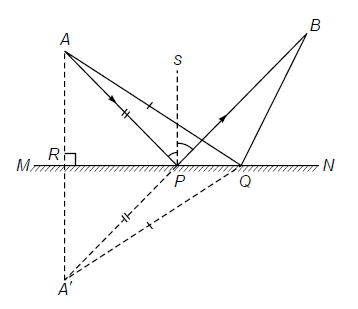
\includegraphics[scale=1]{Figure/9.PNG}
\caption{Law of Reflection}
\end{figure}
\subsubsection{Total Internal Reflection}
\begin{figure}[H]
\centering
\label{fig:12}
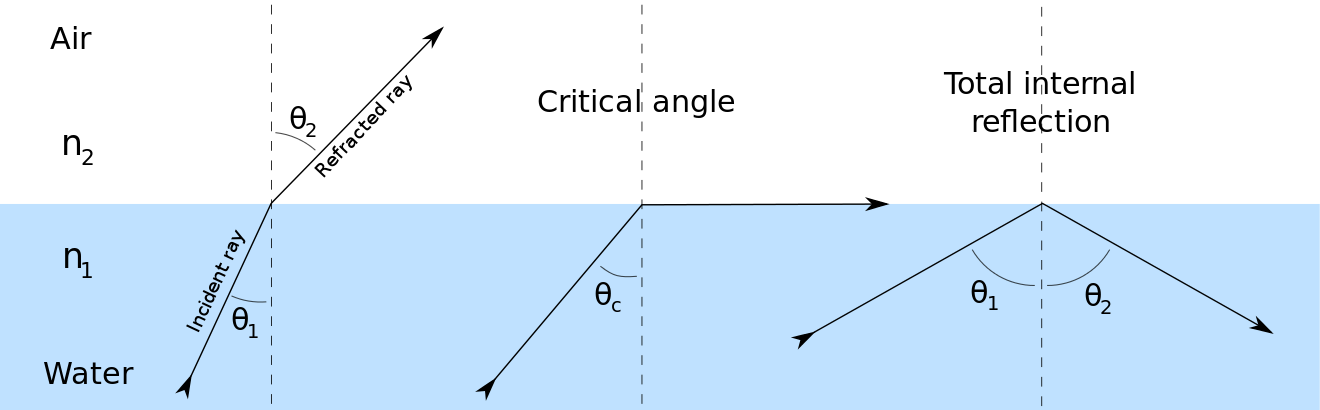
\includegraphics[scale=0.2]{Figure/12.PNG}
\caption{Total Internal Reflection}
\end{figure}
The critical angle: $\theta _c=\arcsin \frac{n_2}{n_1}$

\subsection{Refraction}
\subsubsection{Refraction Index}
\emph{Refraction index}\index{Refraction index} is defined as the ratio between the light speed the wave propagate speed in medium.
\[n=\frac{c}{v}\]
\subsubsection{Snell's Law of Refraction}
\emph{Snell's law of refraction}\index{Snell's law of refraction} states that the light beam or part of it enters a different medium with changed direction corresponding to both refraction index,
\[n_1\sin \theta_1=n_2\sin \theta_2\]
This result follows naturally from both Fermat's principle and Huygen's principle.
\begin{figure}[H]
\centering
\label{fig:10}
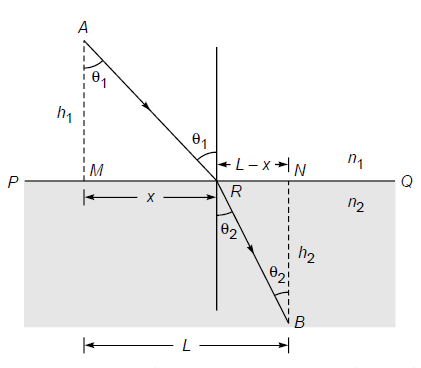
\includegraphics[scale=1]{Figure/10.PNG}
\caption{Snell's Law of Refraction}
\end{figure}
\subsubsection{Dispersion}
An important property of $n$ is that, for a given material, the $n$ varies with the wavelength of the light passing through the material (i.e. Prism) – this behaviour is called \emph{dispersion}\index{Dispersion}.

For example, Light from the source is sent through a narrow, adjustable slit to produce a parallel beam. The light then passes through the prism and is dispersed into a spectrum. 
\[v=\lambda \nu \Rightarrow \frac{\sin \theta _1}{\sin \theta _2}=\frac{n_2}{n_1}=\frac{v _1}{v _2}=\frac{\lambda _1}{\lambda _2}\]

Therefore, for light beam dispersed by prism, blue light has larger blending angle. This is also true for rainbow that the violet strip is outer side respect to the red strip. For double rainbow, the order is reversed.

\subsection{Reflection and Refraction}
\begin{figure}[H]
\centering
\label{fig:13}
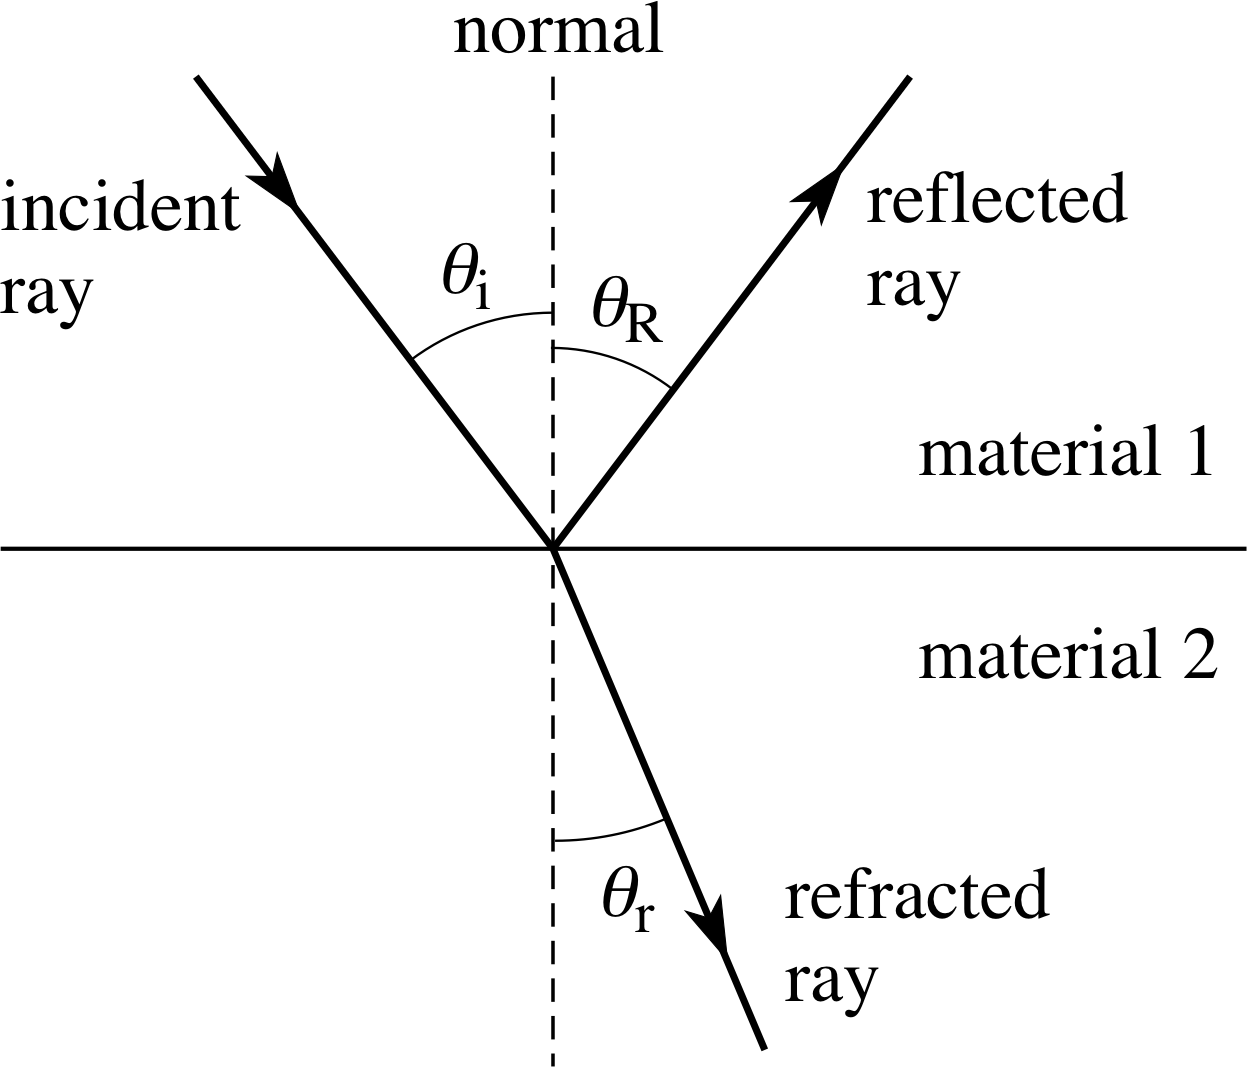
\includegraphics[scale=1]{Figure/13.PNG}
\caption{Reflection and Refraction}
\end{figure}
\section{Polarization}
\emph{Polarization}\index{Polarization} is a property only for transverse waves (not longitudinal).

A beam of light from a normal light source consists of many millions of individual photons and the corresponding vibration axes will be completely random in orientation. The beam as a whole is then \emph{unpolarized}\index{Unpolarized}.

When an atom emits a single photon these fluctuations, within the photon, are \emph{plane polarised}\index{Plane polarised}.

The vibrations in a transverse wave take place at right angles to the direction of propagation, and so are confined to the plane at right angles to this direction.
\subsection{Malus' Law}
If a plane-polarized beam strikes a \emph{polaroid}\index{Polaroid} - polarizing sheet whose axis is at an angle $\theta$q to the incident polarisation direction, the beam will emerge plane-polarized parallel to the Polaroid axis.
\[I=I_0\cos ^2\theta \]

Moreover, the average intensity $\bar{I}=\frac{1}{2}I_0$, since the average of $\cos \theta $
\begin{figure}[H]
\centering
\label{fig:14}
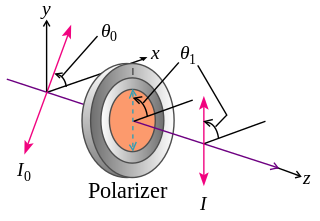
\includegraphics[scale=0.5]{Figure/14.PNG}
\caption{Polarizer ($\theta = \theta _1-\theta _0$)}
\end{figure}
\subsection{Producing Polarized Light}
There are several ways to produce polarized light. As we seen before, polarizer is one equipment you can account to. Besides that
\subsubsection{Reflection ans Scattering}
\begin{figure}[H]
\centering
\label{fig:15}
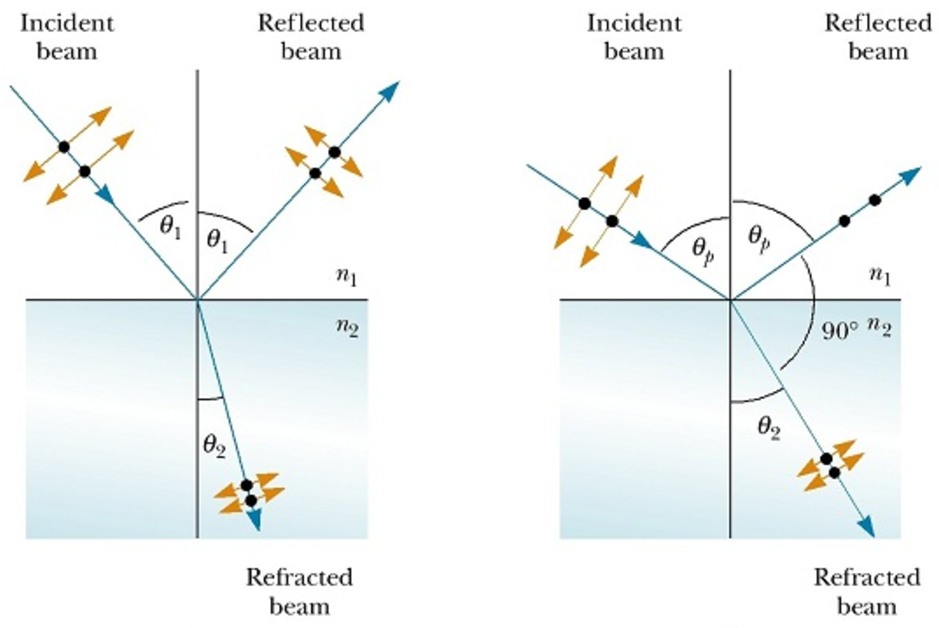
\includegraphics[scale=0.5]{Figure/15.PNG}
\caption{Partially Polarization and Completed Polarization}
\end{figure}
In completed polarization, by \emph{Brewster's law}\index{Brewster's law}, we can determine the Brewster angle $\theta _p$
\[\tan \theta _p=\frac{n_2}{n_1}\]

\begin{proof}
\[\theta _p+\theta _2=\frac{\pi }{2}\]

by the Snell's law, we have
\[n_1\sin \theta _p=n_2\sin \theta _2=n_2\cos \theta _p\]

thus we have the Brewster's law.
\end{proof}
\subsubsection{Double Refraction}
In many crystals, such as quartz and calcite, the polarization direction of the incident light affects the speed at which light travels through the material and hence the material's refractive index $n$, resulting in ordinary (O) ray and extraordinary (E) ray.
\begin{figure}[H]
\centering
\label{fig:16}
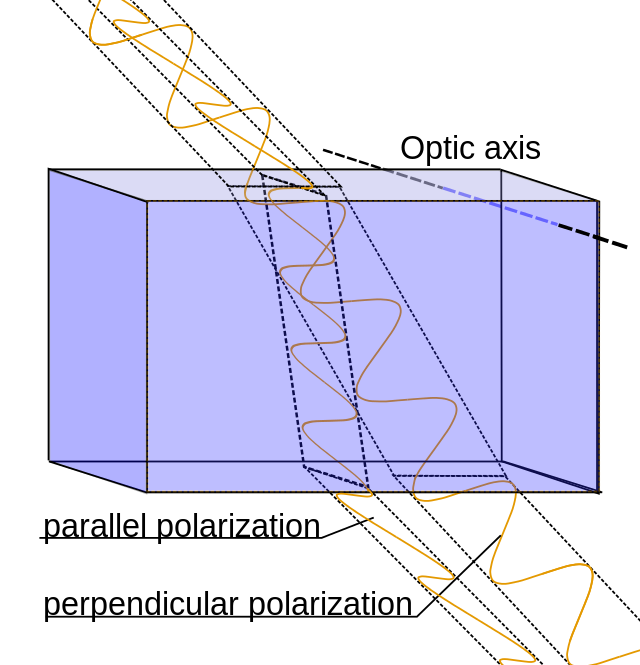
\includegraphics[scale=0.25]{Figure/16.PNG}
\caption{Double Refraction - Birefringence}
\end{figure}
A light beam incident on a crystal will have its two perpendicular components of polarization refracted in different directions.
\subsection{Application of Polarized Light}
\subsubsection{Photoelastic Stress Analysis}
Certain materials only become doubly refracting under stress - \emph{photoelasticity}\index{Photoelasticity}
\subsubsection{Optical Rotation}
Certain materials rotate the plane of polarization by an amount dependent on their thickness or concentration (i.e. organic chirality molecular) - \emph{optical rotation}\index{Optical rotation}
\section{Interference}
\subsection{Superposition Principle}
When two or more waves move in the same linear medium, the net displacement of the medium at any point equals the algebraic sum of the wave functions of the individual waves.
\subsection{Light Wave Interference}
An interference pattern with light is only observable if it is \emph{stationary}\index{Stationary}.

A stationary pattern is only obtained if the
waves involved are \emph{coherent}\index{Coherent}\footnote{Coherent light can be produced be wavefront division (double-slits (Young’s), Lloyd’s mirror) and wave amplitude division (thin film, air-wedge).}

Therefore, in order to get an observable light interference, the following condition must be satisfied:
\begin{itemize}
\item maintain a constant phase difference - coherent
\item have the same frequency - monochromatic
\end{itemize}

\subsection{Wavefront Division}

\paragraph{Young's Double-Slit Experiment}
Young's double-slit experiment is one method of wavefront division. And the interference pattern can be explained by Huygen's principle. 
\begin{figure}[H]
\centering
\label{fig:17}
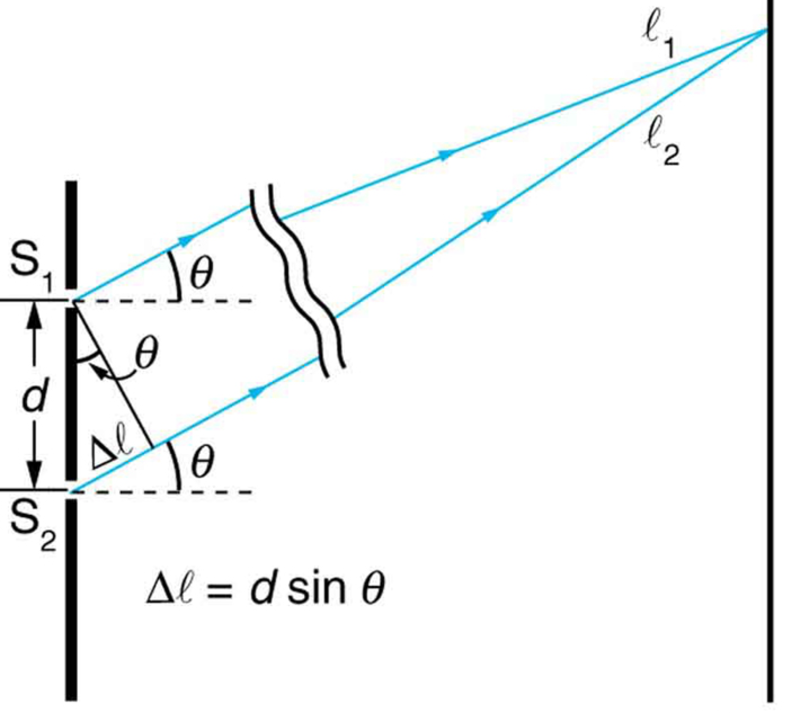
\includegraphics[scale=0.5]{Figure/17.PNG}
\caption{Young's Double-Slit Experiment}
\end{figure}
As the above graph shown, the path difference $\Delta l$ is given by the angle $\theta $ (considered to be small enough), and the slit distance $d$

Furthermore, denote $L$ as the distance between the board and the screen and $y$ as the vertical distance from the center of the screen, and $D$ as the slit width. 
\[\Delta l\approx \sin \theta \]
\[y =L\tan \theta \approx L\sin \theta \]

The approximation is valid if $L\sim 1m$, $D < 1mm$ and $\lambda < 1\mu m$

For the path difference, the two light rays will have a phase difference respect to each. 
\[\phi =\frac{2\pi }{\lambda }\Delta l=\frac{2\pi }{\lambda }d\sin \theta\]

Since the two light rays were divided by the same wavefront, they must have same frequency and amplitude. Therefore, at the point of interference, the two waves can be expressed by:
\begin{align*}
E_1&=E_0\sin \omega t\\
E_2&=E_0\sin (\omega t+\phi )
\end{align*}

by the principle of superposition, the resultant wave is:
\begin{align*}
E&=E_1+E_2=E_0\sin \omega t+E_0\sin (\omega t+\phi )\\
&=2E_0\cos \frac{\phi}{2}\sin \left(\omega t+\frac{\phi}{2}\right)
\end{align*}

And the light intensity will be proportional to the square to the amplitude of the wave. 

Let's look at the location of the dark and bright fringes. For the bright fringe, it is the result of the constructive interference, therefore, at the point of interference, two wave are in phase:
\[\Delta l=d\sin \theta =m\lambda\qquad y_{\textrm{bright}}\approx \frac{m\lambda L}{d} \qquad m\in \mathbb{N}\]

For the dark fringe, it is the result of the destructive interference, therefore, at the point of interference, two wave are $\pi $ out of phase:
\[\Delta l=d\sin \theta =\left(m+\frac{1}{2}\right)\lambda \qquad y_{\textrm{dark}}\approx \left(m+\frac{1}{2}\right)\frac{\lambda L}{d} \qquad m\in \mathbb{N}\]

The average intensity can also be given by the phase difference:
\begin{align*}
I_{\textrm{av}}=I_0\cos ^2\frac{\phi}{2}=I_0\cos ^2 \frac{\pi d\sin \theta}{\lambda}=I_0\cos ^2 \frac{\pi d y}{\lambda L}
\end{align*}

Noted: The central fringe is central maximum, it's a bright fringe.

\paragraph{Lloyd's Mirror}
\begin{figure}[H]
\centering
\label{fig:18}
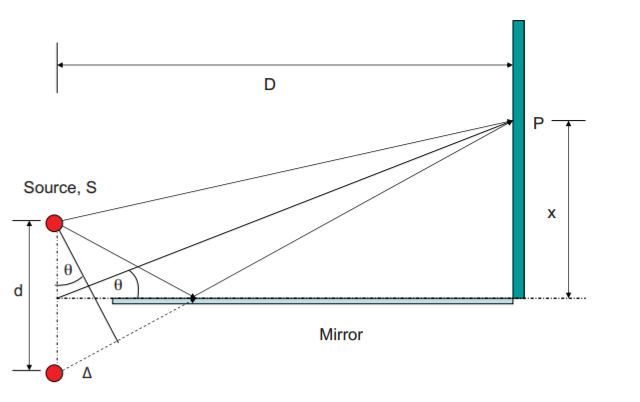
\includegraphics[scale=0.8]{Figure/18.PNG}
\caption{Lloyd's Mirror Experiment}
\end{figure}
Lloyd's mirror can be considered as one method for the wavefront division. Moreover, in this case, the reflected ray will have a $\pi $ phase shift. This phenomenon will happen if light get reflected on the interface of two media and back to the one who has smaller reflected index.

Therefore, taking the phase shift at the interface into account, here is the fringe pattern.

For the bright fringe, it is the result of the constructive interference, therefore, at the point of interference, two wave are in phase:
\[\Delta l=d\sin \theta =\left(m+\frac{1}{2}\right)\lambda \qquad y_{\textrm{bright}}\approx \left(m+\frac{1}{2}\right)\frac{\lambda L}{d}\qquad m\in \mathbb{N}\]

For the dark fringe, it is the result of the destructive interference, therefore, at the point of interference, two wave are $\pi $ out of phase:
\[\Delta l=d\sin \theta =m\lambda \qquad y_{\textrm{dark}}\approx \frac{m\lambda L}{d}\qquad m\in \mathbb{N}\]

And we can see that due to the phase change, the central fringe is a central minimum - a dark fringe. 


\subsubsection{Reflection Phase Change}
An electromagnetic wave undergoes a phase change of $\pi$ upon reflection from a medium that has a higher index of refraction than the one in which the wave is travelling. Why?\footnote{It should account for the conservation and continuity of electromagnetic field along any certain direction at the interface. This phase change is actually a sign flip to maintain the continuity of the wave at boundary and the conserved electromagnetic field.}

This can be shown by the following figure:
\begin{figure}[H]
\centering
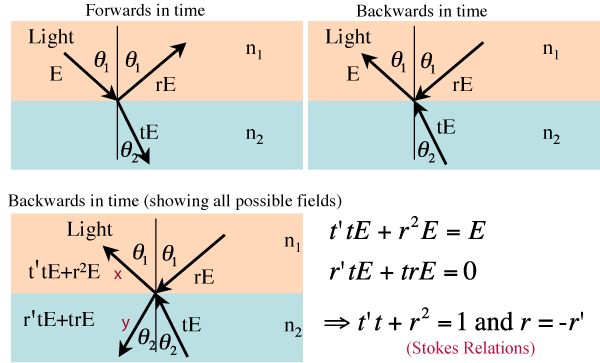
\includegraphics[scale=0.4]{Figure/20.PNG}
\caption{Reflection Phase Change - Stokes Relations (Non-Absorption Process)}
\label{fig:20}
\end{figure}
The most interesting result here is that $r=-r'$. Thus, whatever phase is associated with reflection on one side of the interface, it is $\pi$ different on the other side of the interface. 

\subsection{Division of Wave Amplitude}

\paragraph{Thin Film}
\begin{figure}[H]
\centering
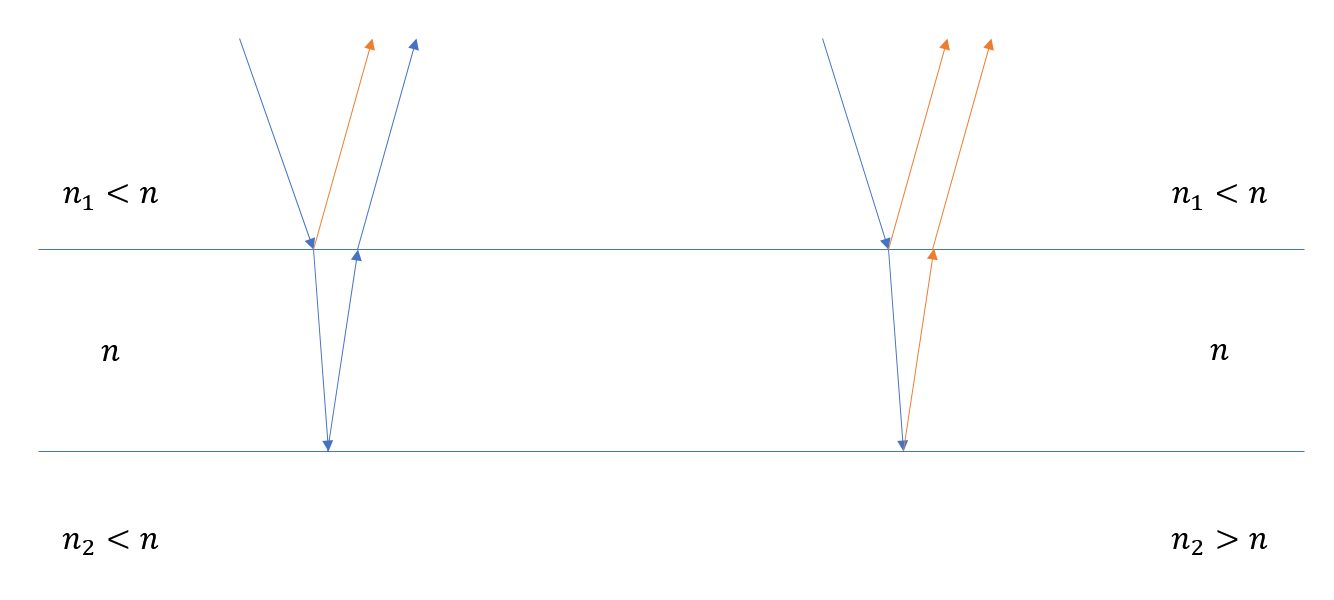
\includegraphics[scale=0.6]{Figure/19.PNG}
\caption{Thin Film}
\end{figure}
In this first case, consider the top surface, the direct reflected beam has a reflection phase change and the beam going through the thin film does not, thus if the width of the thin film $d$ is odd multiples of the quarter of the wavelength $\lambda $ (resulting the path difference is the odd number of half of the wavelength), these two rays will have a constructive interference. And for the case that the width of the thin film is the even multiples of the quarter wavelength (resulting even number of the half wavelength), this two rays will have destructive interference. 

Denote the reflected wavelength as $\lambda _n$. In a medium of refractive index $n$ the wavelength $\lambda _n$ is given by (frequency does not change)
\[\lambda _n=\frac{\lambda }{n}\]

and the path difference is given by
\[\Delta l=\frac{\phi }{2\pi}\lambda\]

therefore, for constructive interference:
\[d = \frac{1}{4}(2m+1)\lambda _n\Rightarrow 2nd=\left(m+\frac{1}{2}\right)\lambda \qquad m\in \mathbb{N}\]

and for the destruction interference:
\[d = \frac{1}{4}(2m)\lambda _n\Rightarrow 2nd=m\lambda \qquad m\in \mathbb{N}\]

For the second case, where two rays are all phase shift by $\pi$, therefore, the phase changes due to reflection at both the top and bottom surfaces are offsetting.
\[\begin{cases}
d = \frac{1}{4}(2m+1)\lambda _n\Rightarrow 2nd=\left(m+\frac{1}{2}\right)\lambda &m\in \mathbb{N} \textrm{ Construction Interference}\\
d = \frac{1}{4}(2m)\lambda _n\Rightarrow 2nd=m\lambda &m\in \mathbb{N} \textrm{ Destruction Interference}
\end{cases}\]

\subsubsection{Fringes of Equal Thickness}
\paragraph{Air Wedge}
This same phenomenon can happen in another experiment - air wedge. 
\begin{figure}[H]
\centering
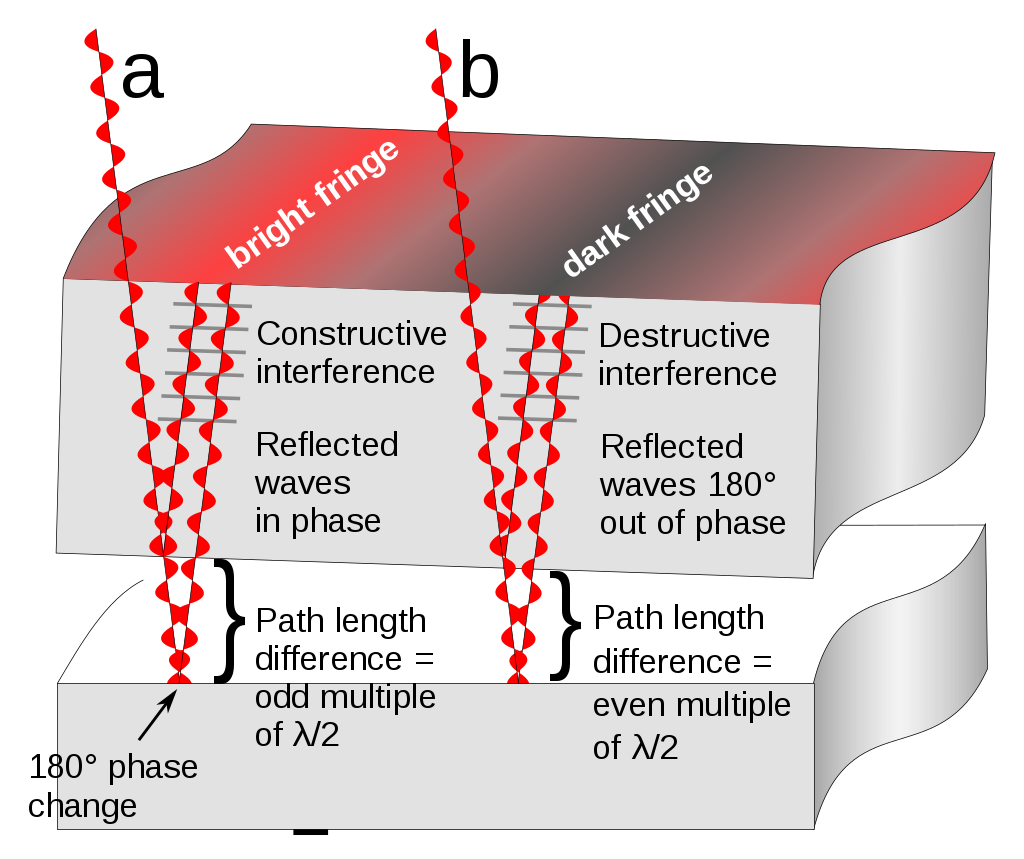
\includegraphics[scale=0.16]{Figure/Air_Wedge_1.PNG}
\caption{Air Wedge}
\end{figure}
Similarly, the conclusion follows:
\[\begin{cases}
d = \frac{1}{4}(2m+1)\lambda _n\Rightarrow 2nd=\left(m+\frac{1}{2}\right)\lambda &m\in \mathbb{N} \textrm{ Construction Interference - Bright Fringe}\\
d = \frac{1}{4}(2m)\lambda _n\Rightarrow 2nd=m\lambda &m\in \mathbb{N} \textrm{ Destruction Interference  - Dark Fringe}
\end{cases}\]

\paragraph{Newton's Ring}

\begin{figure}[H]
    \centering
    \begin{subfigure}[b]{0.45\textwidth}
        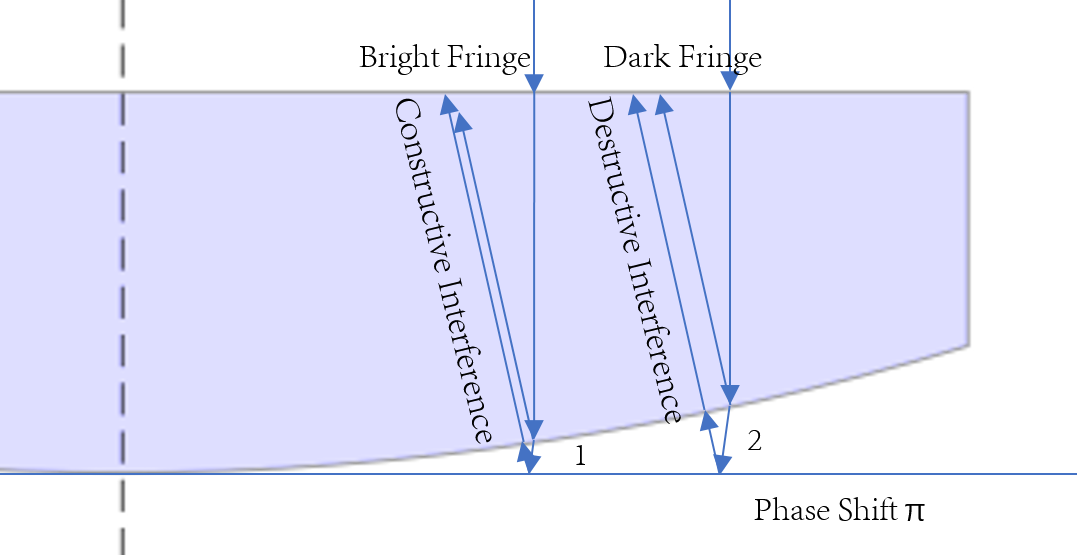
\includegraphics[width=\textwidth]{Figure/Air_Wedge.PNG}
        \caption{Plano-convex lens}
        \label{fig:Plano-convex lens}
    \end{subfigure}
    ~
    \begin{subfigure}[b]{0.45\textwidth}
        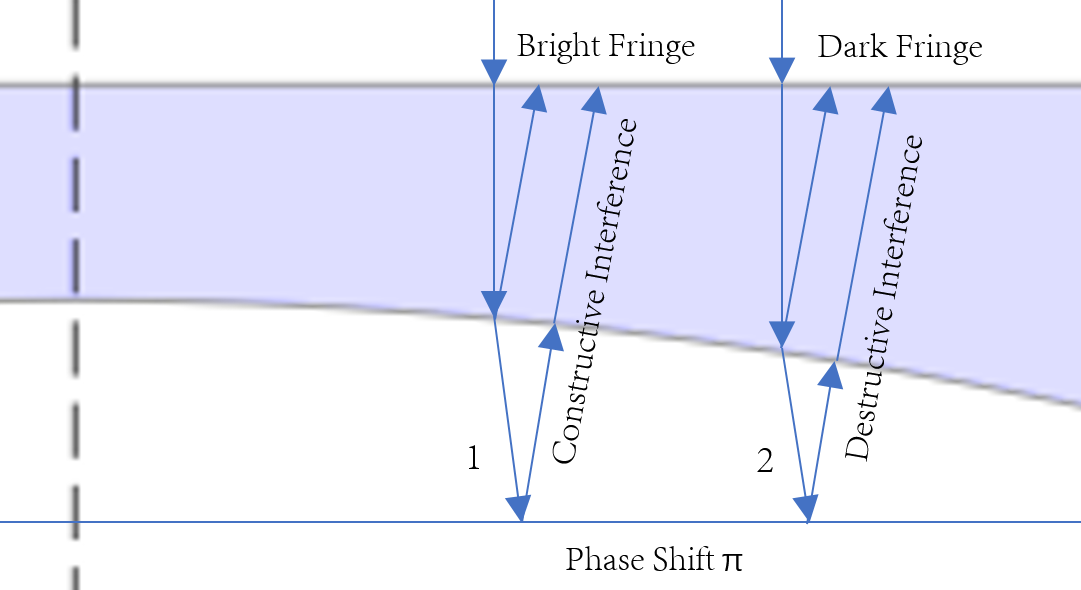
\includegraphics[width=\textwidth]{Figure/Air_Wedge2.PNG}
        \caption{Plano-cylindrical lens}
        \label{fig:Plano-cylindrical lens}
    \end{subfigure}
    \caption{Netwon's Rings}\label{fig:Newton's Rings}
\end{figure}
\emph{Newton's rings}\index{Newton's Rings} is a phenomenon in which an interference pattern is created by the reflection of light between two surfaces — a spherical surface and an adjacent touching flat surface. Basically, it is same as second case in the thin film interference and the air wedge.
\[\begin{cases}
d = \frac{1}{4}(2m+1)\lambda _n\Rightarrow 2nd=\left(m+\frac{1}{2}\right)\lambda &m\in \mathbb{N} \textrm{ Construction Interference - Bright Fringe}\\
d = \frac{1}{4}(2m)\lambda _n\Rightarrow 2nd=m\lambda &m\in \mathbb{N} \textrm{ Destruction Interference  - Dark Fringe}
\end{cases}\]

\begin{wrapfigure}{R}{0.45\textwidth}
  \vspace{-20pt}  
  \begin{center}
    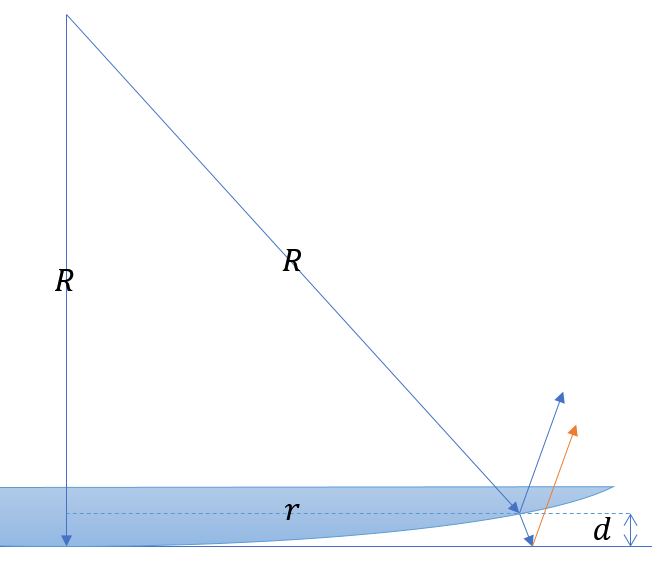
\includegraphics[width=0.4\textwidth]{Figure/21.PNG}
  \end{center}  
  \vspace{-20pt}  
  \caption{Newton's Rings}
  \label{fig:21}
\end{wrapfigure}
Moreover, dark fringe has the radii given by: 
\[r \approx \sqrt{\frac{m\lambda R}{n}}\]
where $n$ is the reflective index of the glass, and $R$ is the distance of the light source to the lower interface at the fringe. For approximation, we assume that the convex lens is part of spherical lens.

\begin{proof}
For the dark fringe, we have the destruction interference, therefore, 
\[2nd=m\lambda \qquad m\in \mathbb{N},\]

Therefore, by the geometrical relation, we have,
\begin{align*}
r&\approx\sqrt{R^2-\left(R-d\right)^2} &\textrm{Spherical lens approximation}\\
&\approx \sqrt{2Rd}&\textrm{Omit the second order }O(d^2)\\
&=\sqrt{\frac{m\lambda R}{n}}&~
\end{align*}
\end{proof}

\subsection{Phasor Diagram}
\begin{wrapfigure}{L}{0.45\textwidth}
  \vspace{-20pt}
  \begin{center}
    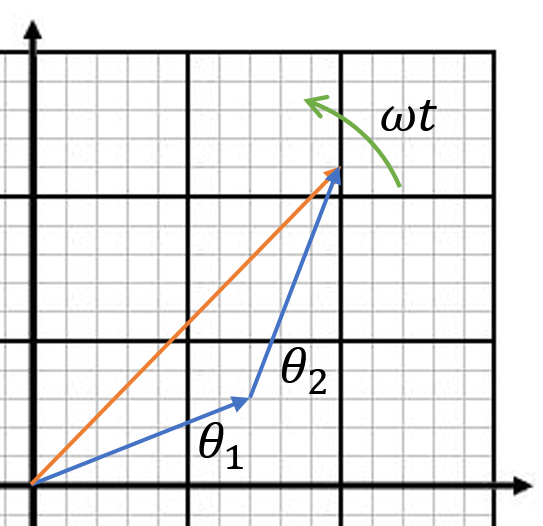
\includegraphics[width=0.4\textwidth]{Figure/Phasor_1.PNG}
  \end{center}  
  \vspace{-20pt}
  \caption{Phasor Diagram}
  \vspace{-40pt}
  \label{fig:Phasor Diagram1}
\end{wrapfigure}
Consider several sinusoidal waves with phase angle difference, we can clearly show the phase difference in a phase diagram:
\begin{align*}
E_1&=E_0\sin \left(\omega t+\theta _1\right)\\
E_2&=E_0\sin \left(\omega t+\theta _2\right)\\
&\vdots\\
E_n&=E_0\sin \left(\omega t+\theta _N\right)
\end{align*}

\subsubsection{Phasor Addition of Waves}
First we can consider the first two sinusoidal waves, as shown by the figure \ref{fig:Phasor Diagram1}, with the length of the phasor represents their amplitudes, we can add them like two vectors and obtain the equivalent total phasor, and that phasor represents the interference wave. Moreover, Consider that the phase difference is $\Delta \theta =\theta _2-\theta _1$, we can calculate:
\begin{align*}
E_1+E_2&=E_0\sin \left(\omega t+\theta _1\right)+A_0\sin \left(\omega t+\theta _1+\Delta \theta \right)\\
&=2E_0\cos \frac{\Delta \theta }{2}\sin \left(\omega t+\theta _1+\frac{\Delta \theta}{2}\right)
\end{align*}

This result is the same as the double slit interference, thus we can generate this result into multiple slit interference.
\subsection{Multiple Slit Interference}
\begin{wrapfigure}{L}{0.32\textwidth}
  \vspace{-20pt}
  \begin{center}
    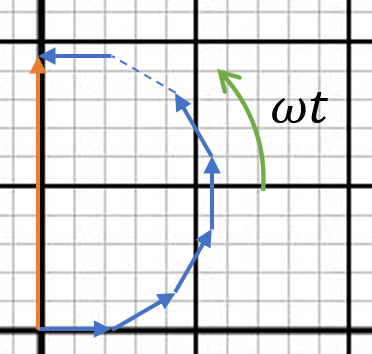
\includegraphics[width=0.3\textwidth]{Figure/Phasor_2.PNG}
  \end{center}  
  \vspace{-20pt}
  \caption{$N$ Slits}
  \vspace{-70pt}
  \label{fig:Phasor Diagram2}
\end{wrapfigure}
Consider there are $N$ slits, dividing same wavefront, thus having same frequency and amplitude. Denotes:
\begin{align*}
E_1&=E_0\sin \left(\omega t+\theta\right)\\
E_2&=E_0\sin \left(\omega t+2\theta \right)\\
&\vdots\\
E_n&=E_0\sin \left(\omega t+N\theta \right)
\end{align*}

In this case, we can get the final results, as 
\[E=\sum _{i=1}^{N}E_i=\underbrace{NE_0\cos \frac{N}{2}\theta }_\text{Interference amplitude}\sin \left(\omega t+\frac{N}{2}\theta\right)\]

Thus we can see that the intensity of interference is $N^2$ as the $I_0$, and we can also see that the secondary maximum has $N-2$ betweem each primary maximum\footnote{This question would be so much easier to understand by taking views of the phasor diagram. For $N$ phasor, there are $N-2$ different polygon that cancel out some phasors and leave the rest to interference as secondary maximum.}.

\subsection{Multiple-Beam Interference (Optional)}
If the amplitude-reflection coefficients, $r$'s, for the parallel plate, are not small, the high-order reflected waves, become quite significant, resulting \emph{multiple-beam interference}\index{Multiple-Beam Interference}.

\begin{figure}[htbp]
\vspace{-10pt}
\centering
\label{fig:22}
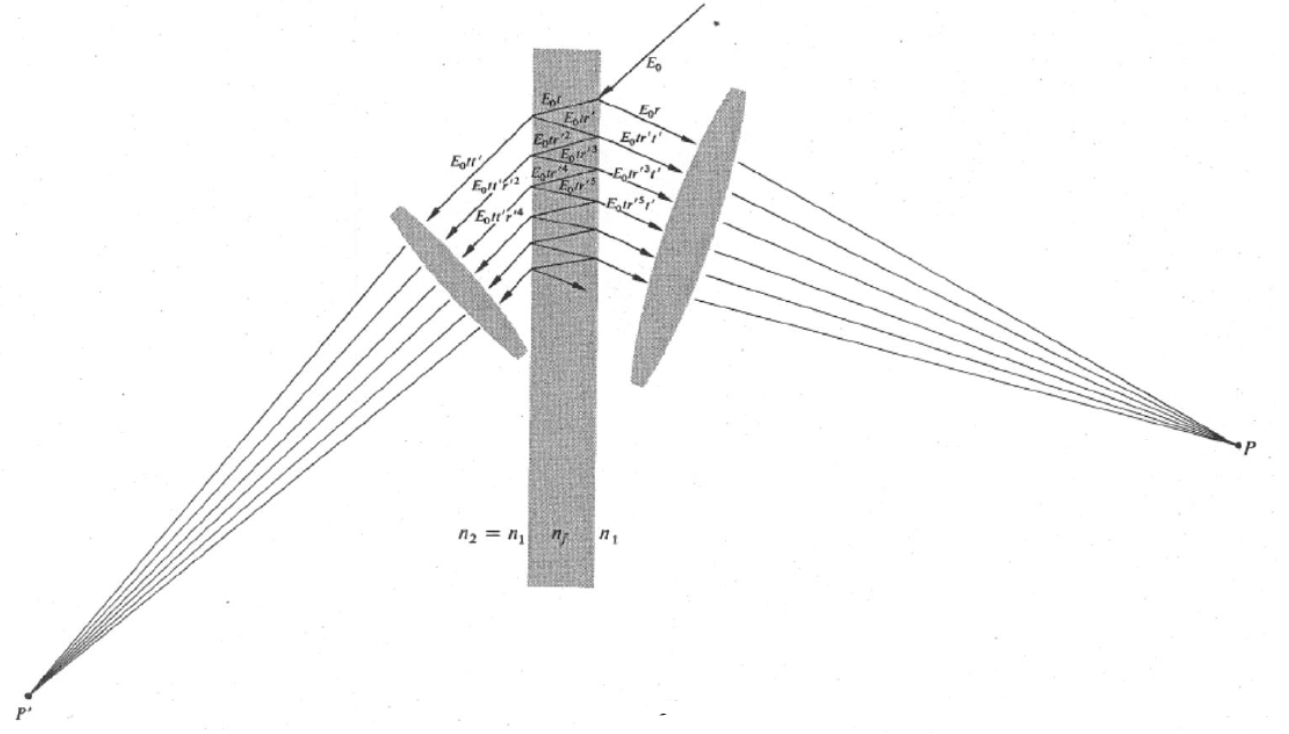
\includegraphics[width=0.9\textwidth]{Figure/22.PNG}
%\vspace{-40pt}
\caption{Multiple-beam interference from a parallel film}
\end{figure}

\begin{wrapfigure}{L}{0.5\textwidth}
  \vspace{-20pt}
  \begin{center}
    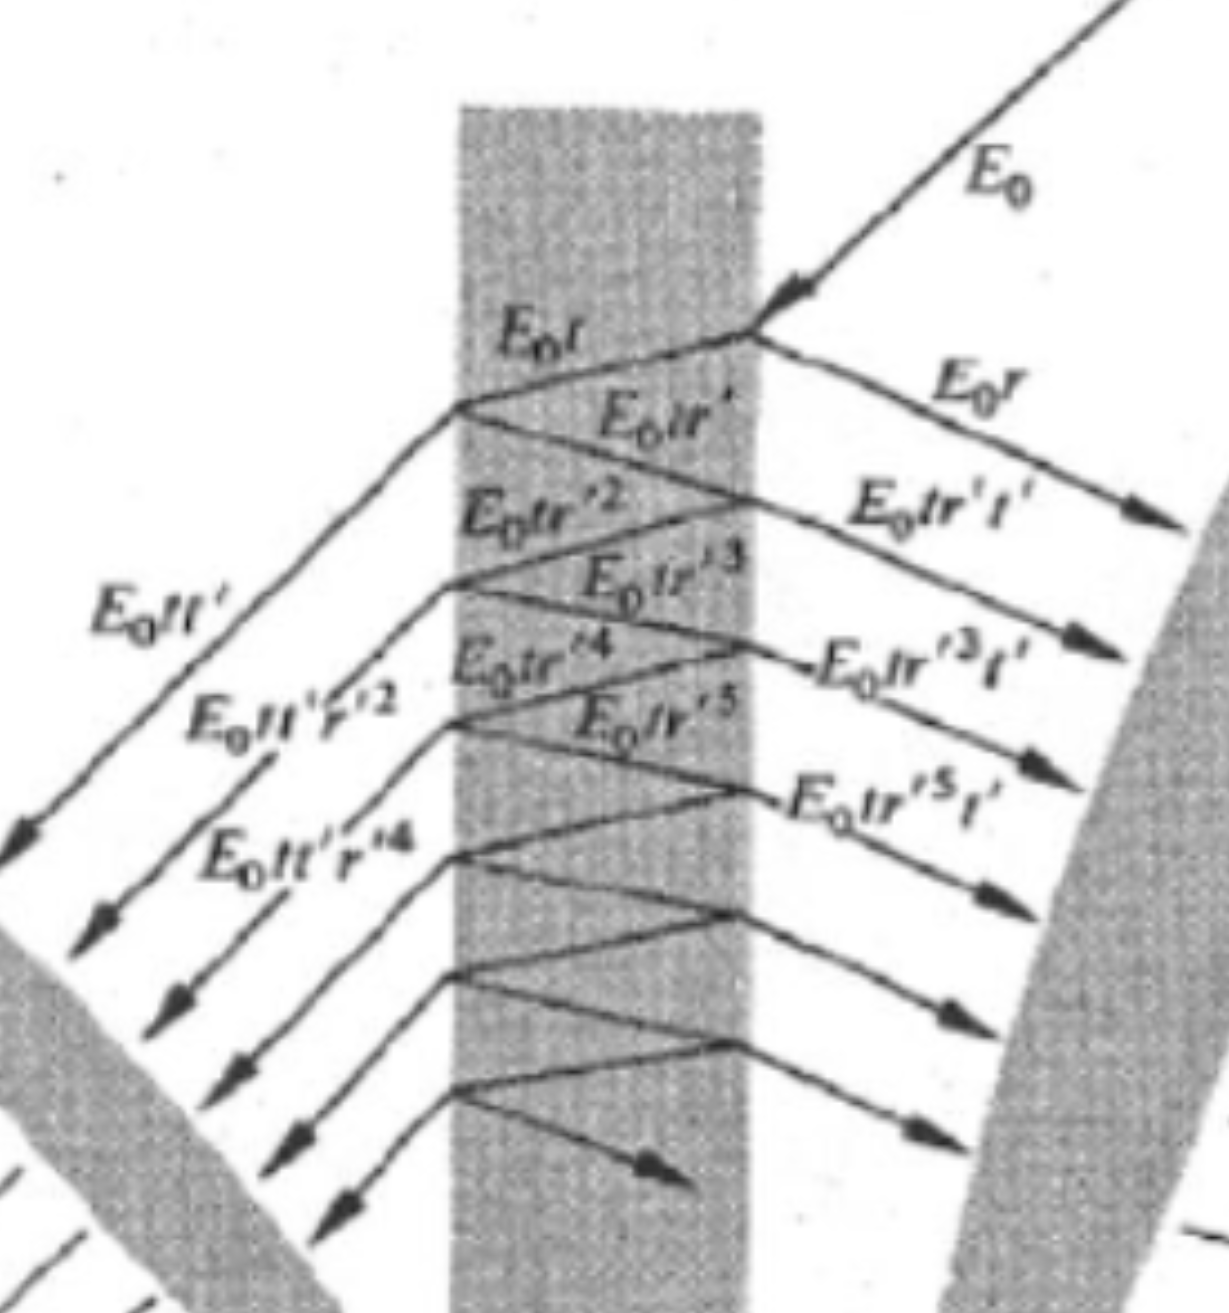
\includegraphics[width=0.45\textwidth]{Figure/23.PNG}
  \end{center}  
  \vspace{-10pt}
  \caption{Reflection and transmission}
  \vspace{-50pt}
\end{wrapfigure}

First, to simplify the question, we make assumptions:
\begin{itemize}
\item The film is non-absorbing.
\item $n_1=n_2$
\item Denote amplitude transmission coefficients: $t$ as entering the film and $t'$ as exiting the film.
\item Denote amplitude reflection coefficient: $t$ as outside the film and $t'$ as within the film.
\item The waves are mutually coherent and will all interfere with the assistance of the lenses.
\end{itemize}

Thus first, we obtain the scalar amplitudes of the reflected waves as $E_{1r},E_{2r},E_{3r},\cdots $ are respectively, $E_0r,E_0tr't',E_0tr'^3t',\cdots $, and the scalar amplitudes of the transmitted waves $E_{1t},E_{2t},E_{3t},\cdots $ are respectively, $E_0tt',E_0tr'^2t',E_0tr'^4t',\cdots$.

The phase differences arise from a combination of the optical path-length differences and phase shifts occurring at the various reflections. 

Between the adjacent rays, the optical path difference is (where $d$ is the width of the parallel film and $\theta _i$ is the incident angle and $\theta _t$ is the transmitted angle)
\[\delta l=2n_fd\cos \theta _t=\frac{\delta }{k_0}\]

Denotes $\delta $ is the phase difference arising from path difference. And $0$ or $\pi $ phase change occurs at each internal reflection ($\theta _i<\theta _c$), thus the optical field at point $P$ are given by:
\begin{align*}
E_{1r}&=E_0re^{i(\omega t+\pi)}\\
E_{2r}&=E_0tr't'e^{i(\omega t+\delta)}\\
E_{3r}&=E_0tr'^3t'e^{i(\omega t+2\delta)}\\
&\vdots\\
E_{Nr}&=E_0tr'^{2N-3}t'e^{i(\omega t+(N-1)\delta)}
\end{align*}

Thus the resultant reflected scalar waves is:
\begin{align*}
E_r&=\sum _{k=1}^{N}E_{kr}\\
&=E_0re^{i(\omega t+\pi)}+E_0tr't'e^{i(\omega t+\delta)}+E_0tr'^3t'e^{i(\omega t+2\delta)}+\cdots +E_0tr'^{2N-3}t'e^{i(\omega t+(N-1)\delta)}\\
&=E_0e^{i\omega t}\left(-r+tr't'e^{-i\delta }\left[\sum _{j=0}^{N-2}\left(r'^2e^{-i\delta}\right)^j\right]\right)\\
&\overset{N\to \infty}{=} E_0e^{i\omega t}\left(-r+\frac{tr't'e^{-i\delta }}{1-r'^2e^{-i\delta }}\right)
\end{align*}

In the case of zero absorption (no loss), $r=r'$and $tt'=1-r^2$ (Stokes Relations\footnote{If you are wonder the sign, I did not flip the sign at the first place :).} ), then
\[E_r=E_0e^{i\omega t}\ \frac{r(e^{-i\delta}-1)}{1-r^2e^{-i\delta}}\]

Therefore, the reflected flux density at $P$ is then $I_r=E_rE_r^*/2$. 
\[I_r=\frac{E_0^2r^2(1-e^{-i\delta })(1-e^{i\delta })}{2(1-r^2e^{-i\delta })(1-r^2e^{i\delta })}=I_i\frac{2r^2(1-\cos \delta)}{(1+r^4)-2r^2\cos \delta}\]

where $I_i$ is the incident flux that $I_i=E_0E_0^*/2=\frac{E_0^2}{2}$

Similarly, we can find the amplitude and irradiance of the transmitted waves\footnote{Proof will be show at appendix.}
\begin{align*}
E_t&=E_0e^{i\omega t}\frac{1-r^2}{1-r^2e^{-i\delta }}\\
I_t&=I_i\frac{(1-r^2)^2}{(1+r^4)-2r^2\cos \delta}
\end{align*}

Let's continuously make analysis for this multi-beam interference:
\begin{align*}
I_r&=I_i\frac{2r^2(1-\cos \delta)}{(1+r^4)-2r^2\cos \delta}&I_{r-max}=I_i\frac{4r^2}{(1+r^2)^2}\\
I_t&=I_i\frac{(1-r^2)^2}{(1+r^4)-2r^2\cos \delta}&I_{t-min}=I_i\frac{(1-r^2)^2}{(1+r^2)^2}
\end{align*}

This gives that: $I_i=I_r+I_t$, coincides with the conservation of irradiance of this given light beam. And we can see that just like the relationship between the kinetic energy and potential energy in spring:
\[\begin{cases}
I_i=I_{r-min}+I_{t-max} &\textrm{ when }\cos \delta =1\textrm{ in which }\delta =2m\pi\\
I_i=I_{r-max}+I_{t-min} &\textrm{ when }\cos \delta =-1\textrm{ in which }\delta =(2m+1)\pi 
\end{cases}\]

\subsection{Fabry-Perot Interferometer}
Based on the principle of multi beam interferometry, \emph{Fabry-Perot interferometer}\index{Fabry-Perot Interferometer}\footnote{The Fabry-Perot etalon is very important in laser technology. The optical resonator in most lasers is a Fabry-Perot interferometer.} consists of two plane glass (or quartz) plates which are coated on one side with a partially reflecting metallic film (of aluminum or silver) of $80\%$ reflectivity.
\begin{figure}[H]
\centering
\label{fig:Fabry-Perot Interferometer}
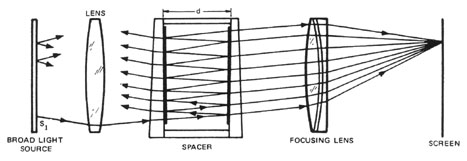
\includegraphics[scale=0.8]{Figure/FIG2.JPG}
\caption{Fabry-Perot Interferometer}
\end{figure}

Light were partially transmitted each time reaches the second surface, resulting in multiple offset beams which can interfere with each other. The large number of interfering rays produces an interferometer with extremely high resolution.

Follow the results in the multi-slit interference, with $tt'=1-r^2$ and $T+R=1$ we have that:
\[I_t=I_i\frac{(1-r^2)^2}{(1+r^4)-2r^2\cos \delta}=I_i\frac{T^2}{1+R^2-2R\cos \delta}\]

Maximum occur when $\cos \delta =1$ in which $\delta =2m\pi $,
\[2n_fd\cos \theta _t=\frac{\delta }{k_0}=\frac{2m\pi }{a\pi /\lambda}=m\lambda \]

As $n_f=1$, we have that $2d\cos \theta _tm\lambda $

\section{Diffraction}
The spreading and bending of wave behind obstacles that lie in their path is called \emph{diffraction}\index{Diffraction}.

The diffraction occurs when the split/object is small enough compared with light wave length.
\subsection{Interference and Diffraction}
Conventionally the term interference is used when considering the intensity pattern produced by superposing a finite number of separated, coherent sources. 

The intensity pattern produced by interference between a continuous distribution of coherent sources is usually called \emph{diffraction}.

\subsection{Fraunhofer and Fresnel Diffraction}
\emph{Fraunhofer diffraction}\index{Fraunhofer diffraction} - rays reaching a point are parallel. Produced either by having large separations between source, obstacle and screen or by using \emph{lenses} (often the eye lens) to focus the rays.

\emph{Fresnel diffraction}\index{Fresnel diffraction} - observing screen is a finite distance from the slit (or edge) and the light rays are not rendered parallel by a lens.

\begin{figure}[H]
\centering
\label{fig:Fresnel diffraction}
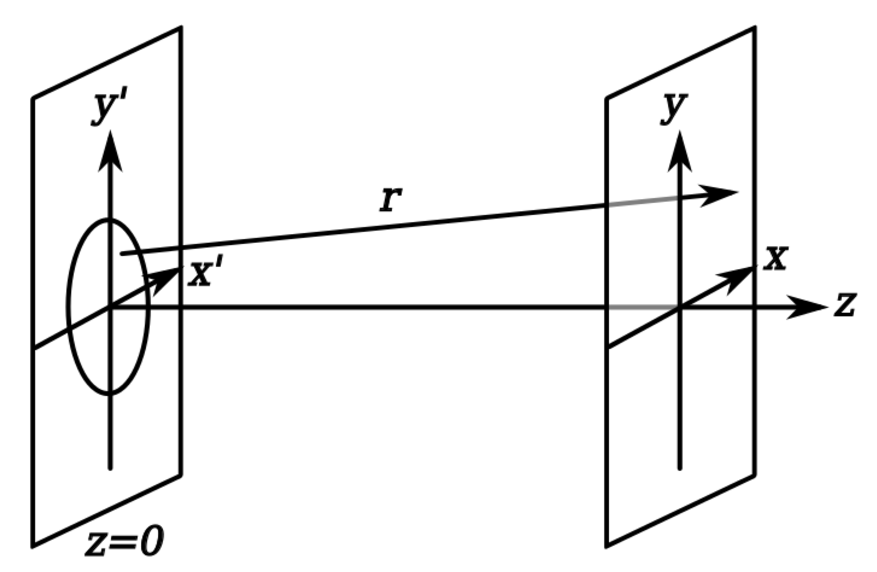
\includegraphics[scale=0.6]{Figure/24.PNG}
\caption{Fresnel diffraction}
\end{figure}

To give you an idea, Fresnel diffraction rises from the Huygen's principle, and its differential equation\footnote{Analytical solution of this integral is impossible for all but the simplest diffraction geometries. Therefore, it is usually calculated numerically.} is the following:

The electric field diffraction pattern at a point $(x, y, z)$ is given by:
\[{\displaystyle E\left(x,y,z\right)={\frac {1}{i\lambda }}\iint _{-\infty }^{+\infty }{E\left(x',y',0\right){\frac {e^{ikr}}{r}}}dx'dy'}\]

where: $E(x',y',0)$ is the aperture, $r =\sqrt{(x-x')^2+(y-y')^2+z^2}$.

In contrast the diffraction pattern in the far field region is given by the Fraunhofer diffraction equation.
\subsection{Single-Slit Diffraction}
In single-slit diffraction, the aperture of the slit can be considered as an array of a large number $N$ of coherent sources, each separated by a small distance $\Delta y$.

\begin{figure}[H]
\centering
\label{fig:Single-Slit Diffraction}
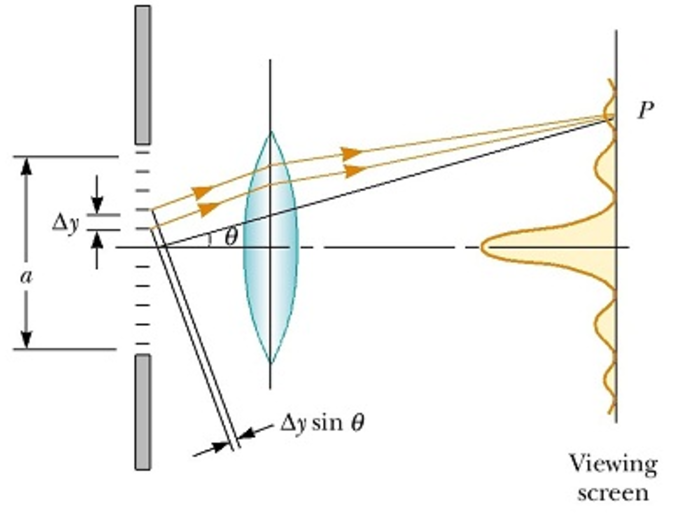
\includegraphics[scale=0.6]{Figure/25.PNG}
\caption{Single-Slit Diffraction}
\end{figure}

Therefore, by making the assumption that the waves are mutually coherent and will all interfere with assistance of the lens. This reduced to a $N$-Slits interference, thus we can use the phasor diagram to solve this question, and then take the limits that $N\to \infty$.

Phasor difference from path difference:
\[\Delta \phi =\frac{2\pi }{\lambda }\Delta y\sin \theta \Rightarrow \phi =N\Delta \phi =\frac{2\pi }{\lambda }N\Delta y\sin \theta \overset{N\Delta y=a}{=}\frac{2\pi }{\lambda }a\sin \theta \]

where $a$ is slit width.

\begin{figure}[H]
\centering
\label{fig:Single-Slit Diffraction1}
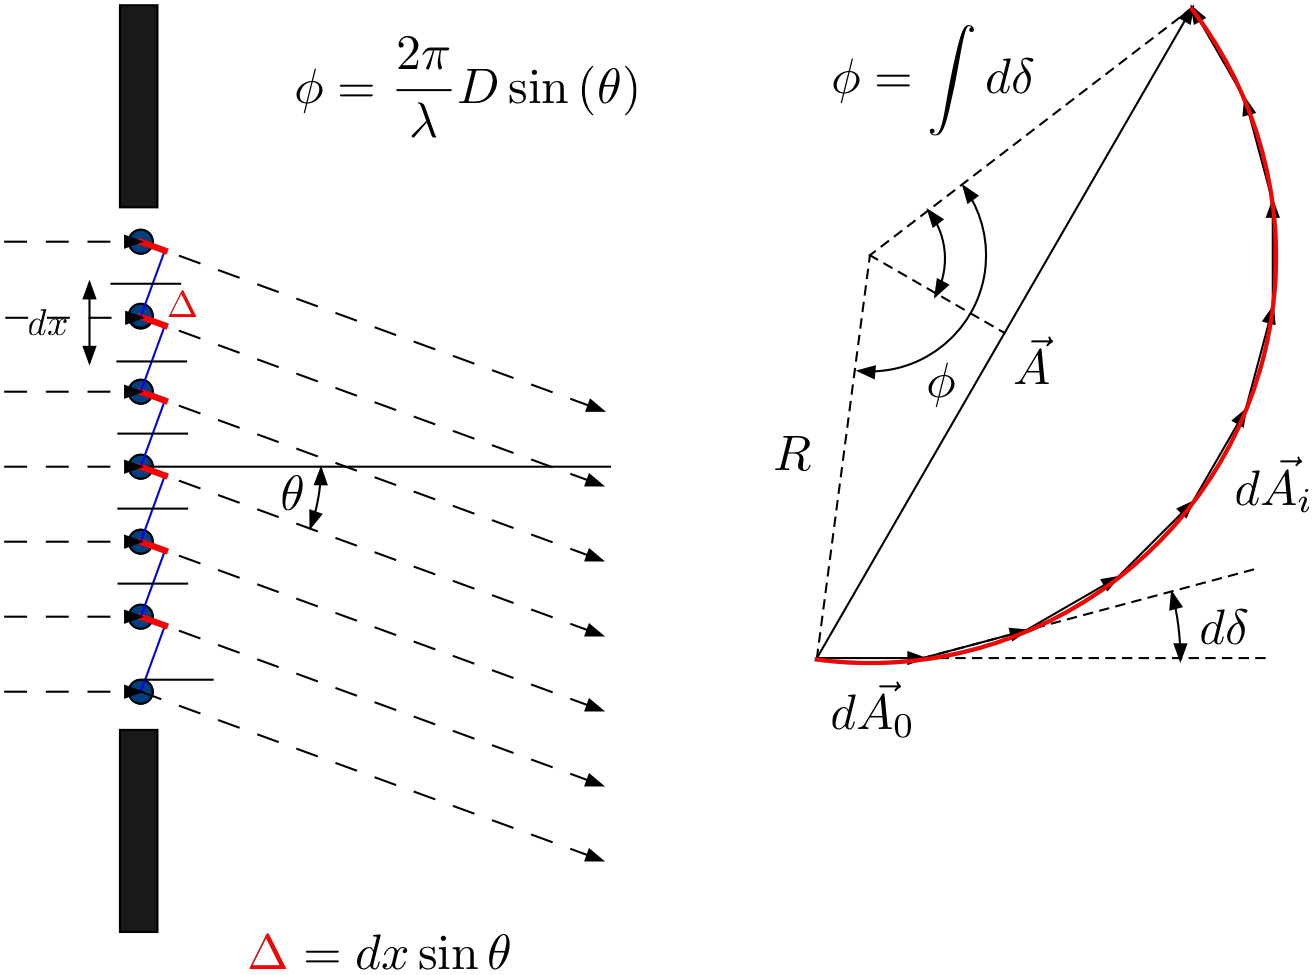
\includegraphics[scale=0.4]{Figure/Phasor_3.PNG}
\caption{Phasor Diagram when $N\to \infty$}
\end{figure}

The total phase difference $\phi $ between the first and last phasors will depends on the angle $\theta $ which determines the direction to an arbitrary point on the screen.

Thinking it as phasor diagram: As $\theta $ increases, the chain of phasors eventually forms the closed path. At greater $\theta $ values, the spiral chain of phasors tightens. And for $N\to \infty$, we will have circled phasor diagram, and the chord is the resultant phasor vector. 

At the same time, for the irradiance, we have that (where $E_R =\vec{A}$):
\[\sin \frac{\phi}{2}=\frac{E_R}{2R}\]

The arc length is $E_0=E\phi $, therefore,
\[E_R=2R\sin \frac{\phi }{2}=E_0\frac{\sin (\phi /2)}{\phi /2}\]

and the irridiance is given by:
\[I_{\theta }=I_0\left(\frac{\sin \frac{\phi}{2} }{\frac{\phi }{2}}\right)^2\]

And we can determine the location of the maximum and minimum. 

Minimum will occur when $\sin \frac{\phi }{2} =0$ but $\phi \neq 0$, therefore, $\frac{\phi}{2} =\pi,2\pi,3\pi,\cdots $, thus the dark fringe will occurs at:
\[\sin \theta =\frac{m\lambda }{a}\qquad m\in \mathbb{N}^+\]

For bright fringe, we have to find that $\phi =0$ (central maximum) and $\tan \frac{\phi }{2}= \frac{\phi }{2}$
\begin{proof}
To obtain the maximum, $\frac{dI}{d\phi }=0$
\[\frac{dI}{d\phi}=\frac{d}{d\phi}I_0\left(\frac{\sin \frac{\phi}{2}}{\frac{\phi }{2}}\right)^2=I_0\frac{\sin \frac{\phi }{2}\cos \frac{\phi }{2}\cdot \frac{\phi }{2}-\sin ^2\frac{\phi }{2}}{(\frac{\phi }{2})^3}=0\]

Thus it requires that $\tan \frac{\phi }{2}= \frac{\phi }{2}$, where $\phi =\frac{2\pi }{\lambda }a\sin \theta$
\end{proof}

For this, we have to solve it numerically to find the bright fringe. Here give the first several solutions of $\frac{\phi }{2}$: $0,\  \pm 1.4303\pi,\  \pm 2.4590\pi,\  \pm 3.4707\pi,\cdots $.

Quick Summary:
\begin{itemize}
\item Minima will occur when $\sin \frac{\phi }{2} =0$ but $\phi \neq 0$, thus $\frac{\phi}{2} =\pi,2\pi,3\pi,\cdots $ and $\sin \theta =\frac{m\lambda }{a}$
\item Maxima will occur when $\phi =0$ (central maximum) and $\tan \frac{\phi }{2}= \frac{\phi }{2}$. Numerically, $\frac{\phi }{2}$: $0,\  \pm 1.4303\pi,\  \pm 2.4590\pi,\  \pm 3.4707\pi,\cdots $.
\end{itemize}
\subsection{Double-Slit Interference and Diffraction Pattern}
As studied, double slits can give interference pattern.
\[I=I_0\cos ^2\frac{\Delta \phi}{2}\]

The interference pattern obtained using slits that are wide enough can produce observable diffraction patterns.

The result gives a superposition of the interference and diffraction patterns.

\begin{figure}[H]
\centering
\label{fig:double slit interference1}
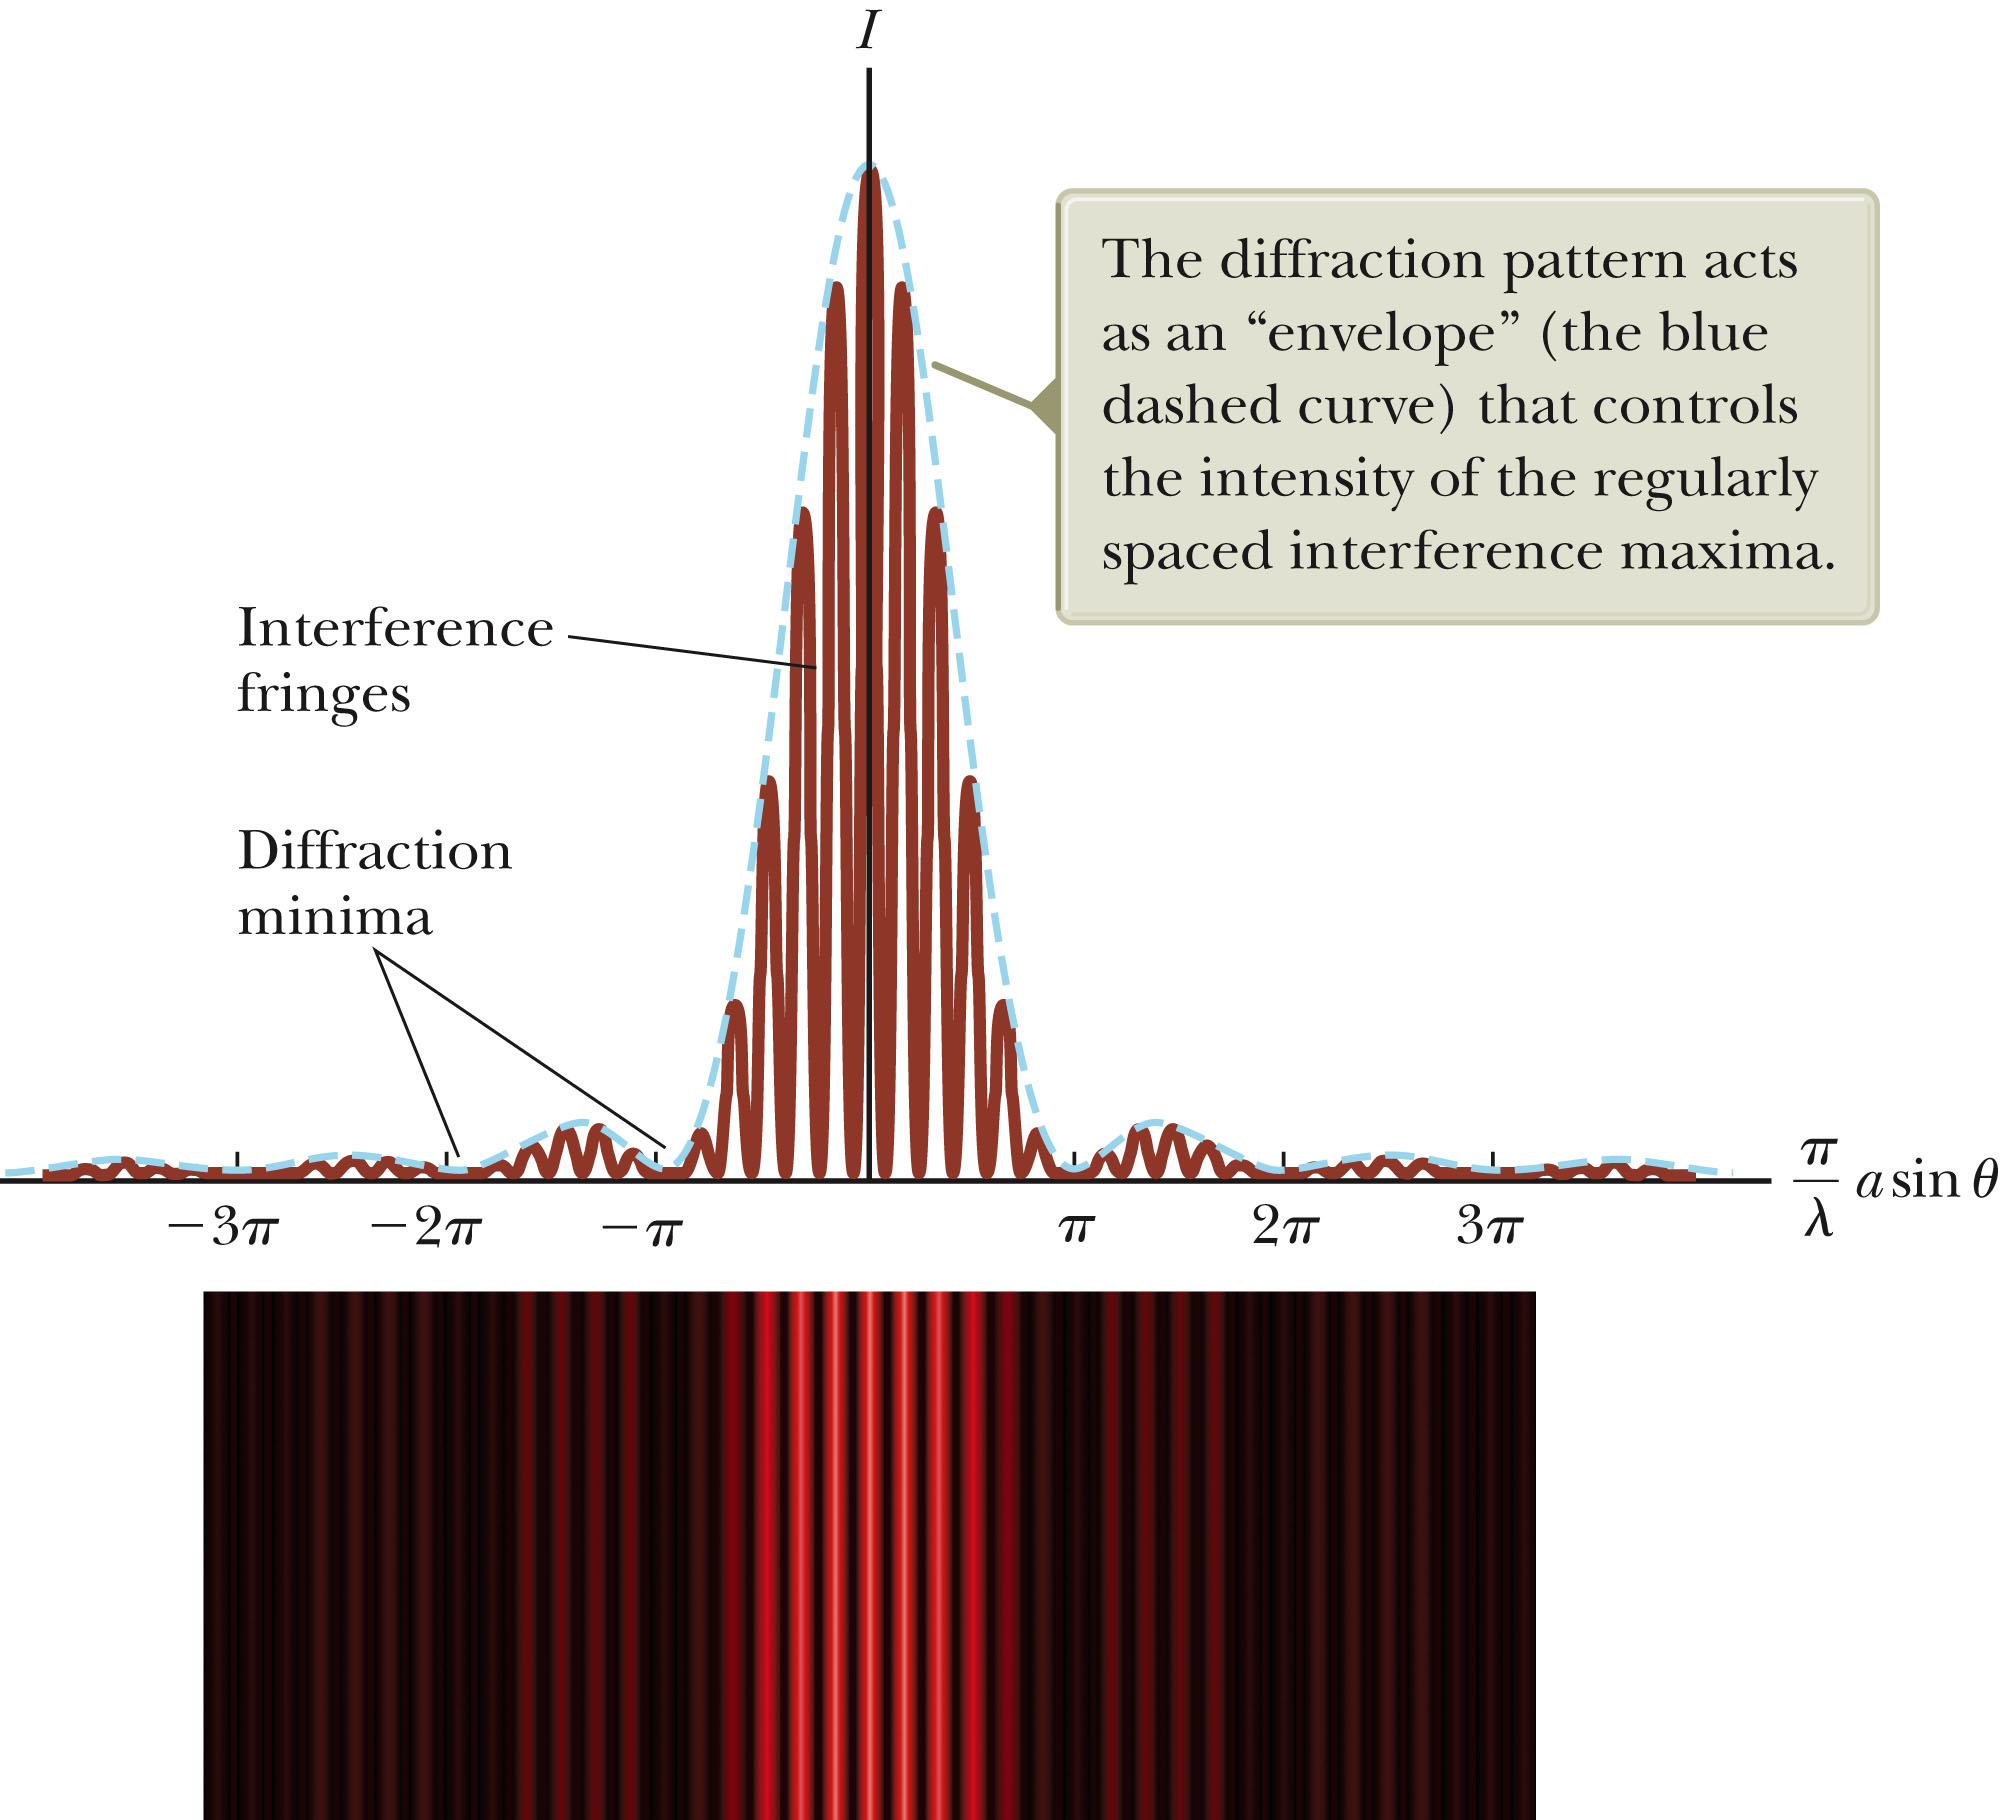
\includegraphics[scale=0.15]{Figure/26.PNG}
\caption{Double Slit Interference and Diffraction}
\end{figure}

Therefore, you can imagine that diffraction curve envelopes the interference, where $d$ is interdistance bewteen two slits, $a$ is the slit width.
\[I=I_0\underbrace{\cos ^2\frac{\pi d\sin \theta}{\lambda }}_\text{Interference}\underbrace{\left[\frac{\sin \left(\frac{\pi }{\lambda }a\sin \theta\right)}{\frac{\pi }{\lambda }a\sin \theta}\right]^2}_\text{Diffraction(envelope)}\]

The result of the superposition of the interference and diffraction.

For double slit interference, the maximum
\[d\sin \theta=m\lambda \]

while for diffraction, the minimum
\[a\sin \theta =\lambda \]

therefore, $m$th ($m=\frac{d}{a}$) maximum will disappear.

\subsection{Diffraction and Image Resolution}
The ability of a lens to produce distinct images of two close objects is called \emph{resolution}\index{Resolution}. Diffraction effects limit this ability.

\begin{figure}[H]
\centering
\label{fig:Diffraction and Image Resolution}
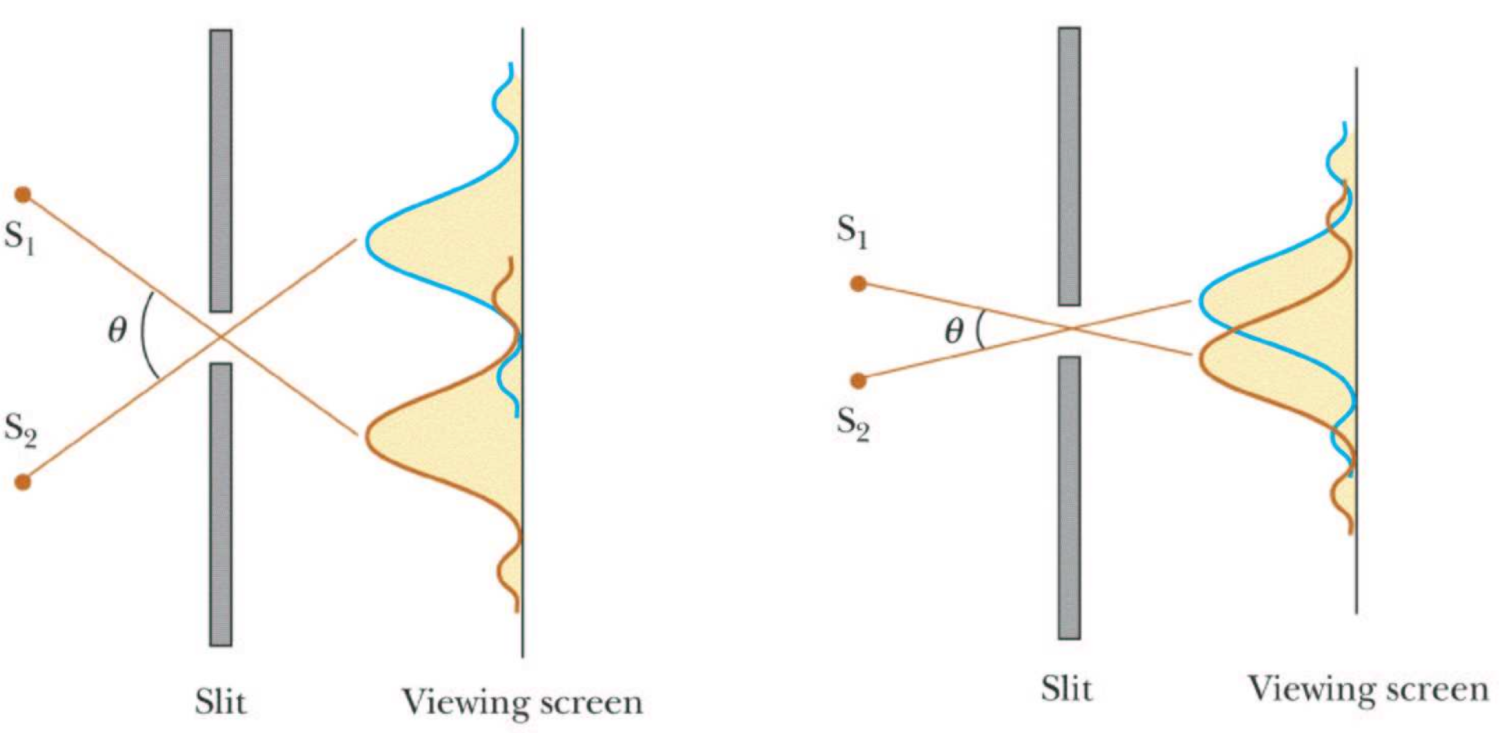
\includegraphics[scale=0.5]{Figure/28.PNG}
\caption{Diffraction and Image Resolution}
\end{figure}

The following showing three definition of the resolutions:
\begin{itemize}
\item The \emph{Rayleigh criterion}\index{Rayleigh criterion} states that the two images will be just resolvable when the centre of the diffraction disc of one falls directly on the first minimum of the diffraction pattern of the other. For a circular aperture
\[\theta =\frac{1.22\lambda }{D}=\frac{1.22}{2n\sin \theta }\]

where $D=2NA$ where $NA$ is  \emph{numerical aperture}\index{Numerical aperture}, and $NA=n\sin \theta $ and $n$ is the index of refraction of the medium being imaged in, and $\theta $ is the half-angle subtended by the optical objective lens.
\item \emph{Abbe criterion}\index{Abbe criterion} stipulates that an angular separation cannot be less than the ratio of the wavelength to the aperture diameter.
\[d = \frac{\lambda}{2NA}\]

\item \emph{Sparrow's resolution limit}\index{Sparrow's resolution limit} is nearly equivalent to the theoretical diffraction limit of resolution, the wavelength of light divided by the aperture diameter, and about $20\%$ smaller than the Rayleigh limit.
\[d = \frac{0.94\lambda }{2NA}\]
\end{itemize}
\begin{figure}[H]
\centering
\label{fig:Diffraction and Image Resolution1}
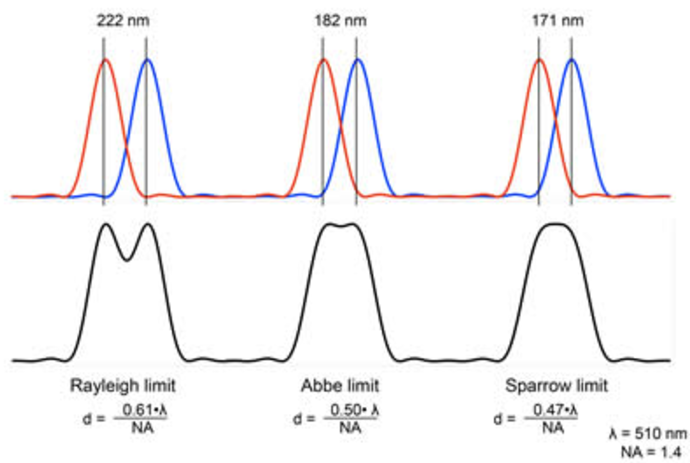
\includegraphics[scale=1]{Figure/27.PNG}
\caption{Three Criterions}
\end{figure}

\subsection{Grating}
Grating is multi-slits interference and diffraction:
\[I=I_0\underbrace{\left(\frac{\sin \alpha}{\alpha}\right)^2}_\text{Diffraction}\underbrace{\left[\frac{\sin N\beta }{\beta }\right]^2}_\text{Interference}\]

where:
\begin{align*}
\alpha &=\frac{\pi }{\lambda }a\sin \theta\\
\beta &=\frac{\pi }{\lambda }d\sin \theta
\end{align*}

and $a$ is the slit width, and the $d$ is the interdistance between two slits.

Interference maxima for: $d\sin \theta=n\lambda $, and diffraction minima for $a\sin \theta =m\lambda $, therefore, just like the double slit diffraction interference pattern, there are some missing order.

Apart from the central maximum, different wavelengths will form images at different angles. The wavelength can be calculated from
\[d\sin \theta _m=m\lambda\]

Images are only found at these defined angles.

If the light consists of a mixture of wavelengths, apart from the central image ($m = 0$), for each order the maxim for different wavelengths will be found at different angles. This forms a spectrum and enables the component wavelengths to be identified.

The number of slits is very large so the number of parallel rays travelling in a direction $\theta $ will also be very large. For the light with the same wavelength, except for phase angle equal zero, at all other angles complete darkness occurs.

\subsubsection{Resolving Power}
The resolving power of a diffraction grating is defined as:
\[R=\frac{\lambda }{\Delta \lambda}\]

where $\lambda =\frac{1}{2}(\lambda _1+\lambda _2)$ and $\Delta \lambda =\lambda _2-\lambda _1$.

This depends only on the order $m$ of the pattern and the number of slits $N$.
\[R=Nm\]
\appendix
\chapter{Electromagnetism}
\section{Energy and Energy Density}
Electromagnetic waves carry energy and can transfer energy to the medium when propagating. The rate of flow of energy in a electromagnetic wave is described by $\mathbf{S}$ defined as: $\mathbf{S}\equiv \mathbf{E}\times \mathbf{H}$

First, consider Faraday's law and Ampere's law in matter,
\begin{align*}
&\nabla \times \mathbf{E}=-\frac{\partial \mathbf{B}}{\partial t}\quad &\textrm{Faraday's Law}\\
          &\nabla \times \mathbf{H}=\mathbf{J}_f+\frac{\partial \mathbf{D}}{\partial t}\quad &\textrm{Ampere's Law} 
\end{align*}
Consider the divergence of $\mathbf{E}\times \mathbf{H}$,
\begin{align*}
\nabla \cdot \left(\mathbf{E}\times \mathbf{H}\right)&=\mathbf{H}\cdot \left(\nabla \times \mathbf{E}\right)-\mathbf{E}\cdot \left(\nabla \times \mathbf{H}\right)\\
&=-\mathbf{H}\cdot \frac{\partial \mathbf{B}}{\partial t}-\mathbf{J}_f\cdot \mathbf{E}-\mathbf{E}\cdot \frac{\partial \mathbf{D}}{\partial t}\\
&=-\left(\mathbf{H}\cdot \frac{\partial \mathbf{B}}{\partial t}+\mathbf{E}\cdot \frac{\partial \mathbf{D}}{\partial t}\right)-\mathbf{J}_f\cdot \mathbf{E}
\end{align*}

and we know that in a linear materials:
\begin{align*}
\mathbf{H}\cdot \frac{\partial \mathbf{B}}{\partial t}+\mathbf{E}\cdot \frac{\partial \mathbf{D}}{\partial t}&=\mu \mathbf{H}\cdot \frac{\partial \mathbf{H}}{\partial t}+\varepsilon \mathbf{E}\cdot \frac{\partial \mathbf{E}}{\partial t}\\
&=\frac{1}{2}\mu \frac{\partial }{\partial t}\left(\mathbf{H}\cdot \mathbf{H}\right)+\frac{1}{2}\varepsilon \frac{\partial }{\partial t}\left(\mathbf{E}\cdot \mathbf{E}\right)\\
&=\frac{1}{2}\frac{\partial}{\partial t}\left(\mathbf{B}\cdot \mathbf{H}+\mathbf{D}\cdot \mathbf{E}\right)
\end{align*}

therefore, we have that $\nabla \cdot \mathbf{S}+\frac{\partial u}{\partial t}=-\mathbf{J}\cdot \mathbf{E}$,  where $\mathbf{S}\equiv \mathbf{E}\times \mathbf{H}$ is known as the \emph{Poynting vector}\index{Poynting vector}, which has physical interpretation of \emph{energy flow}\index{Energy flow}, and $u=\frac{1}{2}\left(\mathbf{B}\cdot \mathbf{H}+\mathbf{D}\cdot \mathbf{E}\right)$, which has the physical interpretation of the energy per unit volume - \emph{wave energy density}\index{Wave energy density}\footnote{This equation is even valid for anisotropic media}.

\chapter{Light Wave Behaviour}
\section{Multiple-Beam Interference}
Prove that the amplitude and irradiance of the transmitted waves are:
\begin{align*}
E_t&=E_0e^{i\omega t}\frac{1-r^2}{1-r^2e^{-i\delta }}\\
I_t&=I_i\frac{(1-r^2)^2}{(1+r^4)-2r^2\cos \delta}
\end{align*}
\begin{proof}
With same assumption and notation, we first obtain the scalar amplitudes of the transmitted waves as $E_{1t}, E_{2t}, E_{3t},\cdots$ are respectively, $E_0tt',E_0tr'^2t',E_0tr'^4t',\cdots $, thus the optical field at point $P'$ are given by:
\begin{align*}
E_{1t}&=E_0tt'e^{i\omega t}\\
E_{2t}&=E_0tr'^2t'e^{i(\omega t+\delta )}\\
E_{3t}&=E_0tr'^4t'e^{i(\omega t+2\delta )}\\
&\vdots\\
E_{Nt}&=E_0tr'^{2N-2}t'e^{i(\omega t+(N-1)\delta )}
\end{align*}

Therefore, the resultant transmitted scalar waves are given by:
\begin{align*}
E_t&=\sum _{k=1}^{N}E_{kt}\\
&=E_0tt'e^{i\omega t}+E_0tr'^2t'e^{i(\omega t+\delta )}+E_0tr'^4t'e^{i(\omega t+2\delta )}+\cdots +E_0tr'^{2N-2}t'e^{i(\omega t+(N-1)\delta )}\\
&=E_0tt'e^{i\omega t}\left(\sum _{j=0}^{N-1}\left[r'^2e^{i\delta }\right]^j\right)\\
&\overset{N\to \infty}{=}E_0tt'e^{i\omega t}\left(\frac{e^{i\delta }}{1-r'^2e^{i\delta }}\right)
\end{align*}

In case of zero absorption (no loss), $r'=r$ and $tt'=1-r^2$ (Stokes Relation\footnote{If you are wonder the sign, I did not flip the sign at the first place :).}), then
\[E_t=E_0\frac{1-r^2}{1-r^2e^{i\delta }}\]

and the irradiance follows $I_t=\frac{E_tE_t^*}{2}$
\[I_t=I_i\frac{(1-r^2)^2}{(1+r^4)-2r^2\cos \delta}\]
\end{proof}
\printindex
\end{document}